\chapter{مروری بر کارهای پیشین}
\newpage
‎\renewcommand{\baselinestretch}{2}\normalsize‎
\label{Previous works}
\section{مقدمه}
در این فصل سعی شده است تا کارهای انجام‌شده و مرتبط با مسائل مطرح شده در این رساله بیان گردد. با توجه به موارد ذکر شده در تعریف مساله، کارهای انجام شده در سه دسته الف) روش‌های یادگیری توزیع‌شده در شبکه‌های تطبیقی و ب) روش‌های یادگیری توزیع‌شده فدرالی و ج) روش‌های موازی‌سازی‌ الگوریتم‌های توزیع‌شده و مدل‌های محاسباتی، مورد بررسی و مطالعه قرار می‌گردند. شبکه‌های تطبیقی توزیع‌شده مقیاس‌پذیر بوده و در برابر خرابی گره‌ها و یال‌ها مقاوم هستند و برای یادگیری مجموعه داده‌های بزرگ با بهره‌مندی از قدرت همکاری میان گره‌ها مناسب می‌باشند. از مدل‌های محاسباتی و روش‌های موازی‌سازی می‌توان در بهبود عملکرد الگوریتم‌های استفاده شده در این نوع شبکه‌ها کمک گرفت. در ادامه، ابتدا به مرور الگوریتم‌های یادگیری ارائه شده در حوزه شبکه‌های تطبیقی توزیع‌شده پرداخته می‌شود، سپس الگوریتم‌های یادگیری فدرالی و در نهایت روش‌های موازی‌سازی  این الگوریتم‌ها و الگوریتم‌های توزیع‌شده مبتنی بر مدل‌های محاسباتی موازی ارائه شده مورد بررسی قرار می‌گیرند.

\section{روش‌های یادگیری توزیع‌شده در شبکه‌های تطبیقی توزیع‌شده}
شبکه‌های تطبیقی در موضوعات مختلفی برای پردازش اطلاعات استفاده می‌شوند. به عنوان مثال رفتارهای پیچیده ظاهر شده در شبکه‌های زیستی و اجتماعی همانند الگوریتم دسته ماهی‌ها، پرواز پرندگان و تعاملات اجتماعی و اقتصادی نمونه‌هایی از این موارد می‌باشند. از شبکه‌های تطبیقی در محیط ایستا و غیرایستا استفاده می‌شود و معمولا هدف در این شبکه‌ها به صورت یک مساله بهینه‌سازی تعریف می‌شود که در آن به دنبال بدست آوردن بردار پارامترهای مجهول با توجه به داده‌های توزیع‌شده در گره‌های مختلف شبکه می‌باشیم. در تخمین متمرکز پارامترها، همه گره‌ها تخمین خود را به گره مرکزی ارسال می‌نمایند. گره مرکزی همه اطلاعات ارسال شده را تلفیق و پردازش می‌نماید. این معماری منابع سیستم از جمله زمان و پهنای باند را هدر می‌دهد و با مشکلات امنیتی و حریم خصوصی داده روبرو است. همچنین در صورتی‌که گره مرکزی با مشکلی روبرو شود، کل سیستم با شکست مواجه خواهد شد. از این رو برای جلوگیری از این مشکلات، پردازش توزیع‌شده مورد توجه محققان قرار گرفته است. 

این روش بر اساس پردازش داده و همکاری‌ها بین گره‌ها پایه‌ریزی شده است و هر گره با استفاده از داده‌هایی که در اختیارش می‌باشد، تخمینی از پارامترهای مجهول ارائه می‌دهد و می‌تواند با توجه به توپولوژی شبکه با همسایه‌هایش تعامل داشته باشد و از آن‌ها اطلاعات دریافت کند و به آن‌ها نیز اطلاعاتی ارسال نماید. بنابراین، پردازش انجام شده مبتنی‌بر داده‌های محلی هر گره و اطلاعات دریافتی از همسایه‌هایش می‌باشد. بر خلاف روش تخمین پارامتر متمرکز، در این روش هیچ مرکز تلفیقی  وجود ندارد. پردازش توزیع‌شده می‌تواند سربار ارتباطی و پردازشی را کاهش دهد. 
اکثر کارهای ارائه‌شده در زمینه برآورد پارامتر از طریق شبکه‌های توزیع‌شده به صورت یک مساله کمینه‌سازی اجماع توابع هزینه هر گره مطرح می‌شوند. گره‌ها با توابع زیان مجزا اما هم مدل در جستجوی یک هدف هستند و نیاز به همگرا شدن به سمت یک پارامتر مشترک دارند. این مسائل تک‌وظیفه‌ای  نامیده می‌شوند.

زمانيكه وروردي فيلتر وفقي نويزي باشد، استفاده از الگوريتم‌هاي مرسوم باعث مي‌شود كارايي فيلتر كاهش‌يافته و تخمين‌هاي آن باياس داشته باشند. در شکل \ref{filter} یک فیلتر تطبیقی با ورودی نویزی نشان داده شده است. روش‌هاي مختلفي براي مقابله با اين مشكل ارائه شده است. در مقاله\cite{Jung2013} روشي براي جبران باياس بر اساس نسخه نرمال \lr{LMS} ارائه شده است تا بتواند اثر منفي نويز ورودي را كاهش دهد. براي حذف باياس نويز ورودي از معياري استفاده شده كه نيازمند تخمين واريانس نويز ورودي است. اما زمانيكه نويز ضربه‌اي باشد، تخمين واريانس نويز چندان موفقيت‌آميز نمي‌باشد. بنابراين براي حل اين مشكل، تخمين واريانس نويز ورودي زمان رخ دادن نويز ضربه‌اي به‌روز خواهد شد. اگر خطا از يك حد مشخصي بيشتر شود، واريانس نويز ورودي مجدد تخمين‌زده مي‌شود و سپس مقدار بردار پارامتر به‌روزرساني مي‌شود. در مقاله \cite{Zheng2017} از الگوريتم حداقل توان چهارم خطا براي بدست آوردن تخميني بدون باياس استفاده شده است. 
\begin{figure}[h]
	\begin{center}
		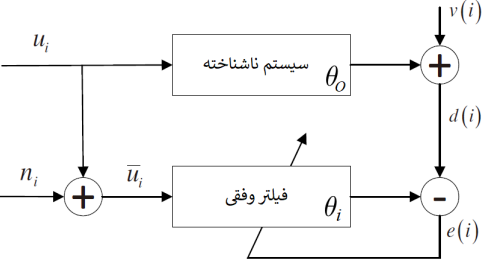
\includegraphics[scale=0.9]{Filter.png}
		\caption{فیلتر تطبيقي با نويز ورودي}
		\label{filter}
	\end{center}
\end{figure}

در شبكه‌هاي تطبيقي توزيع‌شده براي مقابله با مساله نويز ورودي روش‌هايي مختلفی ارائه شده است. شكل \ref{p24} اين مساله را در شبكه‌هاي تطبيقي نشان مي‌دهد. در مقاله \cite{Abdolee2016} روشي بر اساس تخمين واريانس نويز پيشنهاد داده‌اند كه تابع هدف هر گره \lr{k} به صورت زير تعريف مي‌شود:
\begin{equation}\label{e142}
	J_k(w)=E\lvert\lvert d_k(i)-u_{k,i}w\rvert\rvert^2-\sigma^2_{k,i}\lvert\lvert w \rvert\rvert^2
\end{equation}


كه $\sigma_{k,i}^2$ واريانس نويز ورودي در گره $k$ام شبكه است. از الگوريتم انتشار براي حل اين مساله بهينه‌سازي استفاده مي‌شود و روابط به‌روزرساني به‌دست مي‌آيد. اين روش نيازمند تخمين واريانس نويز ورودي است. برخي از كارهاي ارائه شده از توابع زيان پايدارتري براي مقابله با نويز‌هاي ورودي كمك مي‌گيرند. 

\begin{figure}[h]
	\begin{center}
		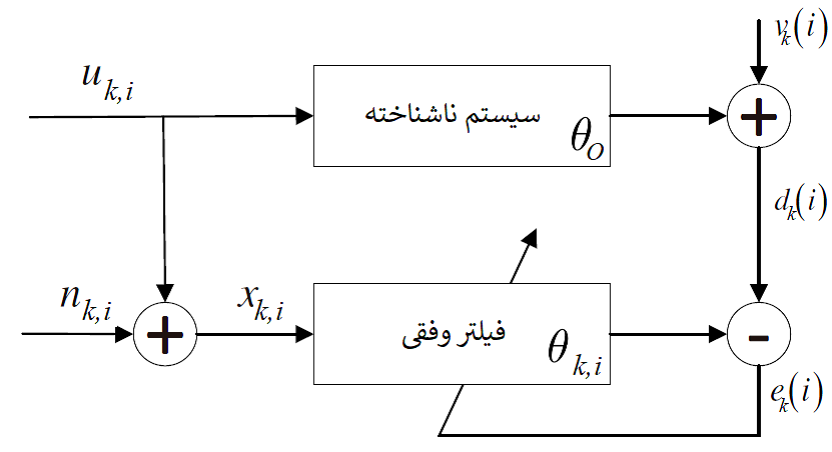
\includegraphics[scale=0.6]{Pic24.png}
		\caption{شبكه تطبيقي با نويز ورودي  \cite{Abdolee2016}}
		\label{p24}
	\end{center}
\end{figure}

كارهاي انجام شده در زمينه مقاوم‌سازي رويكرد‌هاي توزيع‌شده مبتني بر انتشار در برابر نويز را با توجه به تابع هدف مي‌توان به دو دسته الگوريتم‌هاي مبتني بر حداقل‌سازي ميانگين مربعات خطا (\lr{MSE}) و الگوريتم‌هاي مبتني بر مفاهيم تئوري اطلاعات (\lr{ITL}) تقسيم كرد. اگر نويز موجود از مدل گوسي باشد، الگوريتم‌هاي مبتني بر حداقل‌سازي ميانگين مربعات خطا كه به واريانس نويز وابسته هستند، كارآيي مناسبي دارند. اما در برابر نويز غيرگوسي عملكرد مناسبي ندارند و در بعضی مواقع واگرا نيز مي‌شوند. به همين دليل، كارهايي ارائه شده است كه با جايگزين كردن \lr{MSE} با توابع هزينه مقاوم‌تر سعي بر مقابله با نويز‌هاي غيرگوسي دارند. در مقاله \cite{Li2013} الگوريتم حداقل آنتروپي خطا كه يكي از الگوريتم‌هاي مبتني بر تئوري اطلاعات است، بدين منظور استفاده شده است و در آن آنتروپي آخرين \lr{N} نمونه‌اي كه بيشترين ميزان خطا را دارند، به عنوان تابع هدف براي حداقل نمودن خطا استفاده مي‌شود. الگوريتم انتشار معيار حداكثرسازي کورآنتروپی (\lr{DMCC}) \cite{MA2016} از كرنل گوسي به دليل توانايي آن در رد كردن نمونه‌هاي آغشته به نويز غيرگوسي استفاده شده است. تابع هدف اين الگوريتم به صورت زير تعريف مي‌شود:
\begin{equation}\label{e143}
	\begin{cases}
		J_k^{local}(w)=\sum_{l\in N_k}c_{lk} G_{\sigma}(e^2_{l,k})\\
		G_{\sigma}(e^2_{l,k})=\frac{1}{\sigma \sqrt{2\pi}}\exp(-\frac{1}{2\sigma^2}(d_{l,i}-u_{l,i}w_l)^2)
	\end{cases}
\end{equation}

كه $G_{\sigma}(e^2_{l,k})$ تابع استاندارد گوسي با عرض كرنل $\sigma$ است.

الگوريتم‌هاي مبتني بر حداقل‌سازي ميانگين مربعات خطا با تغيير دادن تابع هدف سعي در مقاوم‌سازي در برابر نويز غيرگوسي دارند. الگوريتم انتشار علامت خطا \lr{DSignLMS} \cite{Ni2016} از علامت خطا در تابع هدف استفاده مي‌شود:
\begin{equation}\label{e144}
	\begin{cases}
		J_k^{local}(w)=\sum_{l\in N_k}c_{lk} \lvert\lvert e_{l,k}\rvert\rvert_1\\
		s.t. \lvert\lvert \phi_{k,i}-\theta_{k,i-1}\rvert\rvert^2_2\le\mu_k^2
	\end{cases}
\end{equation}

كه $\phi_{k,i}$ تخمين مياني در گره‌ $k$ام است و بردار گراديان اين الگوريتم به صورت $\nabla J_k^{local}(w)=\sum_{l\in N_k}c_{lk}u_{l,k}sgn(e_{l,k})$ محاسبه مي‌شود. 

در الگوريتم انتشار  \lr{DLMF} \cite{Park2014} ميانگين توان چهارم خطا در تابع هدف براي مقابله با نويز غيرگوسي به كارگرفته شده است. همچنين در الگوريتم انتشار \lr{RDLMS} \cite{Ashk} از تابع زيان شبه‌هابر\footnote{\lr{Pseudo-huber}} بدين منظور استفاده شده است. در \cite{Bert2011} روش‌هايي براي مقابله با داده‌هاي نويزي در الگوريتم \lr{RLS} مطرح شده است. 

الگوريتم‌ها و رويكرد‌هايي كه تاكنون براي شبكه‌هاي تطبيقي توزيع‌شده مطرح‌شده‌‌اند، با فرض داشتن محیط همزمان عمل مي‌كردند. با در نظر گرفتن اتفاقات تصادفي همچون زمان ورود داده‌ها، خرابي گره‌ها و لينك‌ها، تغييرات توپولوژي شبكه و غیره، در مقاله \cite{Zhao2014} پياده‌سازي الگوريتم انتشار با رويكرد \lr{ATC} به صورت زير در محيط غیرهمزمان ارائه شده است.
\begin{equation}\label{e145}
	\begin{cases}
		\psi_k(i)=w_k(i-1)-\mu_k(i) \nabla_{w^T}J_k({w_k(i-1)})\qquad(Adapt)\\
		w_k(i)=\sum_{l\in N_{k,i}}a_{lk}(i)\psi_l(i)\qquad(Combine)
	\end{cases}
\end{equation}
كه در رويكرد غیرهمزمان $\mu_k(i)$ و $a_{lk} (i)$ با زمان تغییر می‌کنند و $N_{k,i}$ مجموعه همسایگی گره $k$ در زمان $i$ را بیان می‌کند. 

به عنوان جمع‌بندی این بخش، در شکل \ref{p11} دسته‌بندی الگوریتم‌های مبتنی بر انتشار برای مقابله با چالش‌های موجود در شبکه‌های تطبیقی نشان داده شده است. این دسته‌بندی براساس سه دیدگاه انجام شده است: الف) تک وظیفه‌ای و چندوظیفه‌ای ب) روش‌های همزمان و غیرهمزمان ج) تابع هدف. در یادگیری تک وظیفه‌ای همه گره‌ها به‌دنبال تخمین یک بردار پارامتر مشترک هستند و باهم همکاری می‌کنند \cite{Lop2008}. درحالی‌که در یادگیری چند وظیفه‌ای هر گره یا زیرمجموعه‌ای از گره‌ها بردار پارامتر مطلوب خود را دارند \cite{Chen2014}. مدل‌سازی، مقاومت و تحلیل کارآیی این الگوریتم‌ها خارج از حوزه این رساله است. به دو دیدگاه دسته‌بندی دیگر در مباحث قبلی به طور کامل اشاره شده‌ است.

\begin{figure}[h]
	\begin{center}
		\includegraphics[scale=0.55]{Pic111.png}
		\caption{دسته‌بندی الگوریتم‌های تطبیقی مبتنی بر انتشار \cite{Ashk}}
		\label{p11}
	\end{center}
\end{figure}

روش‌ها و استراتژي‌های مختلفی برای یادگیری و بهینه‌سازی در شبکه‌های تطبيقي توزیع‌شده ارائه‌ شده است. با توجه به اينكه مباحث همگرایی \footnote{\lr{Convergence}}  و عملکرد این الگوریتم‌ها چالش برانگیزتر از اجرا و پیاده‌سازی روش‌های همکارانه، غیرهمکاری و متمرکز است، مطالعات زيادي در اين زمينه انجام شده است. مي‌توان به مفاهيمي همانند نقطه مجاز\footnote{\lr{Limit point}}، پايداري\footnote{\lr{Stability}}، نرخ يادگيري\footnote{\lr{Learning rate}} و كارآيي\footnote{\lr{Performance}}   در اين شبكه‌ها اشاره كرد.‌ نقطه مجاز یعنی هر گره کجا همگرا مي‌شود، پایداری یعنی تحت چه شرایطی همگرایی رخ مي‌دهد، نرخ یادگیری یعنی با چه سرعتی همگرایی اتفاق مي‌افتد، و کارایی یعنی چقدر گره‌ها به نقطه مجاز نزدیک شده‌اند. برخي از اين مفاهيم در مقالات \cite{Kha2012, Haj2018, Sayed2014} نيز مورد مطالعه قرار گرفته‌اند. 

\section{روش‌های یادگیری توزیع‌شده فدرالی}
یادگیری فدرال (\lr{FL})\footnote{\lr{Federated Learning}} به مدل‌های بصری (\lr{visual}) امکان می‌دهد تا با استفاده از داده‌های دنیای واقعی دستگاه‌های تلفن همراه با حفظ حریم خصوصی آموزش داده شوند. با توجه به ماهیت توزیع‌شده دستگاه‌ها و عملکرد کاربران آن‌ها، آمار داده‌ها در این دستگاه‌ها احتمالاً به طور قابل توجهی متفاوت است. در حالی که در آموزش مرکز داده\footnote{\lr{Data-center training}}، دسته‌های داده معمولاً می‌توانند \lr{IID} (مستقل و دارای توزیع یکسان) فرض شوند، اما این فرض در تنظیمات یادگیری فدرال بعید است. در چند سال گذشته، ابزارهای یادگیری فدرال برای پرداختن به آموزش‌های توزیع‌شده در مقیاس بزرگ در بسیاری از دستگاه‌ها یا گره‌ها، با قابلیت‌های حفظ حریم خصوصی در مقایسه با سیستم‌های یادگیری ماشین توزیع‌شده (\lr{DML})، استفاده شده‌اند. الگوریتم‌های یادگیری فدرالی به جای اشتراک‌گذاری داده‌های خام مانند یادگیری ماشین توزیع‌شده به تبادل نمونه‌های آموزش‌دیده محلی و پارامترهای یادگیری ماشین همچون وزن‌ها و بایاس‌های شبکه‌ عصبی متکی هستند. 

مساله بهینه‌سازی ضمنی در یادگیری فدرالی با عنوان بهینه‌سازی فدرالی  اشاره می‌شود. بهینه‌سازی فدرالی چندین ویژگی کلیدی دارد که آن را از یک مساله بهینه‌سازی توزیع‌شده معمول متمایز می‌کند. 
\begin{itemize}
	\item 
	\lr{Non-IID}: داده های آموزشی در یک کلاینت معین معمولاً بر اساس استفاده از دستگاه تلفن همراه توسط یک کاربر خاص است و از این رو مجموعه داده محلی هر کاربر خاص نماینده توزیع جمعیت نخواهد بود.
	\item 
	\lr{Unbalanced}: برخی از کاربران نسبت به سایرین از سرویس یا برنامه سنگین‌تری استفاده می‌کنند که منجر به مقادیر متفاوتی از داده‌های آموزشی محلی می شود.
	\item 
	\lr{Massively distributed}: انتظار  داریم تعداد کلاینت‌هایی که در یک بهینه‌سازی شرکت می‌کنند بسیار بیشتر از میانگین تعداد نمونه‌های هر مشتری باشد.
	\item
	\lr{Limited communication}: دستگاه‌های تلفن همراه اغلب آفلاین یا دارای اتصالات کند و گران هستند.
\end{itemize}

کاربردهای عملی زیادی از ایده کلی یادگیری فدرال وجود دارد. دو تنظیمی که ممکن است به طور قابل توجهی بر طراحی الگوریتم‌های عملی تأثیر بگذارد به شرح زیر می‌باشند:
\begin{itemize}
	\item 
	یادگیری فدرالی بین دستگاهی یا \lr{Cross-device}: در این نوع، یادگیری ماشین با استفاده از جمعیت زیادی از دستگاه‌های موبایل مورد نظر است.
	\item 
	یادگیری فدرالی بین سازمانی یا \lr{Cross-silo}: در این نوع، یادگیری مشارکتی بین چندین سازمان مورد هدف است.
\end{itemize}

هر دو تنظیم دارای ناهمگنی داده‌ها، محاسبات و همچنین محدودیت‌های ارتباطی و حریم خصوصی هستند، اما تفاوت‌های ظریفی نیز دارند. تنظیمات بین دستگاهی و بین سازمانی عمدتاً توسط محدودیت‌های تحمیلی سیستم تعریف می‌شوند و تنها دو مورد از بسیاری از روش‌های ممکن یادگیری فدرال می‌باشند. این دو تنظیم به دلیل کاربرد زیاد و پذیرش عملی آنها توسط صنعت تا به امروز موضوع بسیاری از تحقیقات در مورد یادگیری فدرال بوده‌اند. دیگر سناریوهای یادگیری فدرال شامل شبکه‌هایی هستند که در آن‌ها ارتباطات بسیار مطمئن با تأخیر کم ضروری است. وسایل نقلیه در جاده، یا به طور کلی شبکه‌های لبه بی‌سیم نمونه‌ای از این شبکه‌ها می‌باشد. در ادامه تفاوت‌های این دو تنظیم مورد بررسی قرار گرفته‌اند.
\begin{itemize}
	\item 
	\textbf{تعداد کلاینت‌ها}: تعداد کل کلاینت‌ها در یادگیری فدرال بین دستگاهی معمولاً بسیار بیشتر از یادگیری فدرال بین سیلو است. تعداد کلاینت‌ها (سازمان‌ها) در یادگیری فدرال بین سیلو می‌تواند به اندازه دو، اغلب ده‌ها یا صدها باشد، در حالی که تعداد کلاینت‌ها‌ (دستگاه‌ها) در یادگیری فدرال بین دستگاهی می‌تواند به راحتی از میلیون‌ها دستگاه فراتر رود. مقدار داده‌های خصوصی در هر مشتری در یادگیری فدرال بین دستگاهی می‌تواند کمتر از یادگیری فدرال بین سیلو باشد. این ممکن است بر ناهمگنی داده‌ها تأثیر بگذارد.
	\item 
	\textbf{دردسترس بودن کلاینت‌ها}: کلاینت‌های بین سیلو معمولاً در مراکز داده نگهداری می‌شوند، که به معنای در دسترس بودن بالا است که احتمالاً همه مشتریان را قادر می‌سازد در هر دور شرکت کنند. در مقابل، جمعیت زیاد با در دسترسی متناوب در یادگیری فدرال بین دستگاهی نشان می‌دهد که سرور فقط می‌تواند از طریق برخی از فرآیندهای نمونه‌برداری به مشتریان دسترسی داشته باشد و سرور فقط توانایی محدودی برای کنترل آن دارد. در تنظیمات بین دستگاهی، در دسترس بودن مشتری برای شرکت در آموزش ممکن است با توزیع داده‌های آموزشی محلی آن نیز مرتبط باشد و تغییرات روزانه را معرفی کند که الگوریتم‌های بهینه‌سازی ممکن است به آن نیاز داشته باشند.
	\item 
	\textbf{توپولوژی اتصال}: اتصالات همتا به همتای مستقیم (غیر از سرور) معمولاً در پلتفرم‌های دستگاه موبایل به خوبی پشتیبانی نمی‌شوند، در حالی که در تنظیمات بین سیلو، چنین اتصالات مستقیم مشتری به مشتری ممکن است آسان‌تر باشد. در یادگیری فدرالی بین سیلو، محققان انواع الگوهای ارتباطی از قبیل یادگیری فدرالی غیرمتمرکز، یادگیری فدرالی افقی، یادگیری فدرالی سلسله‌مراتبی و یادگیری تقسیم‌شده را بررسی کرده‌اند.
	\item
	\textbf{محدودیت‌های ارتباطی و محاسباتی}: محدودیت‌های محاسباتی و ارتباطی در تنظیمات بین دستگاهی سخت‌تر هستند. دستگاه اغلب محاسبات و قدرت ارتباطی محدودی دارند، در حالی که کلاینت‌ها در تنظیمات بین سیلو اغلب می‌توانند مراکز داده‌ای باشند که قادر به استقرار شتاب‌دهنده‌های سخت‌افزاری و پیوندهای ارتباطی با پهنای باند بالا هستند.
	\item 
	\textbf{حالت محاسبات محلی-کلاینت}: با توجه به جمعیت زیاد، اهداف حفظ حریم خصوصی در سطح کلاینت و ضرورت نمونه‌گیری، در تنظیمات بین دستگاهی، ممعمولاً فرض می‌شود که دستگاه‌ها هیچ شناسه‌ای ندارند و ممکن است فقط یک بار در کل فرآیند آموزشی شرکت کنند. بنابراین، در این تنظیمات، الگوریتم‌های بدون \lr{client-side state} به طور کلی ضروری هستند. در مقابل، از آنجایی که اکثر مشتریان در اکثر دوره‌های آموزش بین سیلو شرکت می‌کنند، الگوریتم‌های \lr{stateful} مناسب هستند.
\end{itemize}

یادگیری فدرالی از لحاظ وجود یا عدم وجود یک سرور مرکزی در معماری شبکه مورد استفاده به دو دسته اصلی یادگیری فدرالی متمرکز و غیرمتمرکز تقسیم می‌شوند. در ادامه‌ی این بخش به طور مفصل روش‌های توزیع دادها، انواع یادگیری فدرالی و الگوریتم‌های آن‌ شرح داده می‌شوند.
\subsubsection{روش‌های توزیع‌ داده‌ها در یادگیری فدرال}
برای مطالعه بهینه‌سازی فدرال، باید نحوه توزیع داده‌ها بر روی کلاینت‌ها را مشخص کنیم. در مقاله \cite{Fed1} دو روش برای پارتیشن‌بندی داده‌های \lr{MNIST} روی کلاینت‌ها بررسی شده است: \lr{IID}، که در آن داده‌ها به‌هم ریخته می‌شوند، و سپس بین 100 مشتری تقسیم می‌شوند که هر کدام 600 نمونه دریافت می‌کنند، و \lr{Non-IID}، که در آن ابتدا داده‌ها را بر اساس برچسب رقمی مرتب می‌شوند، آن به 200 قسمت با اندازه 300 تقسیم می‌شوند. و به هر 100 کلاینت 2 زیرمجموعه اختصاص داده می‌شود. این یک پارتیشن‌بندی \lr{Non-IID} از داده‌ها است، زیرا اکثر کلاینت‌ها تنها نمونه‌هایی از دو رقم را خواهند داشت. بنابراین، می‌توان درجه شکست الگوریتم‌ها را در داده‌های \lr{Non-IID} بررسی کرد. به این روش حالت \lr{ sort-and-partition } گفته می‌شود. در \cite{Fed2} به طور مشابه پارتیشن‌های بسیار زیادی بر روی مجموعه داده \lr{CIFAR-10 } تولید کرده و جمعیتی متشکل از 10 کلاینت در مجموع تشکیل داده شده است. این تنظیمات تا حدودی غیر واقعی هستند، زیرا یادگیری فدرال عملی معمولاً شامل مجموعه بزرگتری از کلاینت‌ها با توزیع‌های پیچیده‌تر از پارتیشن‌بندی‌های ساده است. در برخی دیگر از مقالات توزیع داده‌های واقعی‌تر در کلاینت‌ها استفاده شده است. 

در مقاله \cite{Fed3} مجموعه داده \lr{EMNIST} با پارتیشن‌بندی بر روی نویسندگان ارقام به جای پارتیشن‌بندی ساده بر روی کلاس ارقام استفاده شده است. در مقاله \cite{Fed4} توزیع دریکله با پارامتر غلظت 0.5 برای ترکیب کردن مجموعه داده‌های غیریکسان استفاده می‌شود. به طور مشابه، مقاله \cite{Fed5} یک محدوده پیوسته از پارامتر غلظت در توزیع دریکله را با کاوش دقیق در تنظیمات بهینه‌سازی و هایپرپارامتر بهینه جستجو می‌کند. نویسندگان برای ترکیب جمعیتی از کلاینت‌های غیریکسان را از توزیع دیریکله ترسیم می‌کنند، که $p$ توزیع کلاس قبلی را روی $N$ کلاس مشخص می‌کند، و $α > 0$ پارامتر غلظتی است که یکسانی را در بین کلاینت‌ها کنترل می‌کند. زمانیکه $\alpha\to \inf$، تمام کلاینت‌ها دارای توزیع یکسانی با قبلی هستند و زمانیکه $\alpha\to 0$ هر کلاینت شامل نمونه‌هایی از یک کلاس است که به صورت تصادفی انتخاب شده‌اند.

\subsubsection{یادگیری فدرالی متمرکز}
یادگیری فدرال متمرکز یک الگوی یادگیری ماشین توزیع‌شده است که در آن تعداد زیادی از گره‌ها با یک سرور مرکزی هماهنگ می‌شوند تا یک مدل را بدون به اشتراک گذاشتن داده‌های آموزشی خود یاد بگیرند. در این الگوریتم‌ها داده‌های خام گره‌ها هرگز با سرور یا سایر گره‌ها به اشتراک گذاشته نمی‌شود. این امر یادگیری فدرال را از بهینه‌سازی توزیع‌شده سنتی متمایز می‌کند و نیاز به رقابت با داده‌های ناهمگن دارد. در مفهوم اساسی یادگیری فدرال، به دنبال کمینه‌سازی تابع هدف هستیم. تابع هدف یادگیری فدرالی در رابطه زیر آورده شده است. 

\begin{equation}\label{e115}
	\begin{cases}
		\min_{w\in R^d} f(w)=\frac{1}{P} \sum_{i=1}^{|p|}F_i(w)\\
		F(w)=E_{i\sim P}[F_i(w)], \qquad  where \quad F_i(w)=E_{\xi\sim D_i}[f_i(w,\xi)]
	\end{cases}
\end{equation}
که $w\in R^d$ پارامتر مدل عمومی را نشان می‌دهد و $F_i: R^d\to R$ تابع هدف محلی در گره $i$ است. $P$ یک توزیع روی جمعیت گره‌ها است. تابع خطا محلی در گره $i$ یعنی $f_i(w,\xi)$ اغلب برای تمام گره‌ها یکسان است اما توزیع داده محلی $D_i$ اغلب متفاوت خواهد بود. انواع الگوریتم یادگیری فدرالی متمرکز در ادامه شرح داده شده است.

\subsubsection{الگوریتم \lr{FedSGD}}
در الگوریتم یادگیری \lr{FedSGD} یک کسر $C$ از گره‌ها در هر دور انتخاب شده و گرادیان تابع خطا روی تمام داده‌های نگه‌داری شده توسط این گره‌ها محاسبه می‌شود. در واقع پارامتر $C$ اندازه دسته داده کلی را کنترل می‌کند. به صورتی که $C=1$ معادل گرادیان کاهشی \lr{full-batch} بدون حالت تصادفی (\lr{non-stochastic}) است. گرادیان‌های محاسبه شده به سرور مرکزی ارسال می‌شوند و سرور مرکزی گرادیان‌ها را تجمیع کرده و رابطه به‌روزرسانی زیر را بر روی مدل کلی اعمال می‌کند:
\begin{equation}\label{e116}
	w_{t+1}=w_t-\eta \sum_{k=1}^K \frac{n_k}{n}g_k
\end{equation}
که $K$ تعداد گره‌هایی را نشان می‌دهد که داده‌ها روی آنها پارتیشن‌بندی شده‌اند. با توجه به اینکه $P_k$ مجموعه اندیس داده‌ها بر روی گره $k$ را نشان می‌دهد، $n_k=|P_k|$ تعداد داده‌های موجود در گره $k$ و $n=\sum_{k\in K} n_k$ تعداد کل داده‌ها را نشان می‌دهند. 

\subsubsection{الگوریتم \lr{FedAvg}}
در الگوریتم یادگیری \lr{FedAvg} یک کسری از گره‌ها در هر دور انتخاب شده و هر گره انتخاب شده به صورت محلی یک گام از گرادیان کاهشی بر روی مدل جاری و با استفاده از داده‌های محلی خودش اجرا می‌کند. هنگامی که الگوریتم به این صورت نوشته شود، می‌توانیم با تکرار به‌روزرسانی محلی، محاسبات بیشتری به هر گره اضافه کنیم. 
\begin{equation}\label{e117}
	w_{t+1}^k=w_t-\eta g_k
\end{equation}
و سپس سرور مدل‌های محلی دریافت شده از گره‌ها را تجمیع کرده و با استفاده از رابطه \ref{e118} که یک میانگین وزن‌دار از مدل‌های نتیجه شده است، مدل عمومی را به‌روزرسانی می‌کند:
\begin{equation}\label{e118}
	w_{t+1}=\sum_{k=1}^K \frac{n_k}{n}w_{t+1}^k
\end{equation}

در مقاله \cite{Fed1} بر روی خصوصیات \lr{unbalanced} و \lr{Non-IID} تاکید شده است. یک طرح به‌روزرسانی همزمان که در دورهایی (\lr{round}) از ارتباطات پیش می‌رود. یک مجموعه ثابتی از \lr{K} گره با مجموعه داده‌های محلی ثابت خودشان وجود دارد. در ابتدای هر دور یک کسر تصادفی $C$ از گره‌ها انتخاب شده و سرور پارامترهای مدل جاری عمومی را برای گره‌های انتخاب شده ارسال می‌کند. هر گره انتخاب شده محاسبات محلی را بر اساس مدل عمومی و داده‌های محلی خودش اجرا می‌کند و سپس به‌روزرسانی‌ها به سرور ارسال می‌شوند. سرور این به‌روزرسانی‌ها را به مدل عمومی اعمال می‌کند و این فرآیند تا رسیدن به همگرایی مورد نظر ادامه می‌یابد. نویسندگان مقاله نشان می‌دهند که با استفاده از داده‌های \lr{MNIST} الگوریتم \lr{FedAvg} بر روی گره‌ها با توزیع غیریکسان داده‌ همچنان به دقت $\%99 $ همگرا می‌شود، اگرچه دور‌های بیشتری را نسبت به گره‌ها با توزیع یکسان داده انجام می‌دهد.

\subsubsection{الگوریتم \lr{FedAvgM}}
الگوریتم \lr{FedAvg} از \lr{vanilla SGD} در سرور استفاده می‌کند در حالی که الگوریتم \lr{FedAvgM} از \lr{SGD} با پارامتر تکانه $0.9$ بر روی سرور استفاده می‌کند. رابطه به‌روزرسانی در سرور مرکزی با استفاده از رابطه \ref{e119} انجام می‌شود \cite{Fed5}.

\begin{equation}\label{e119}
	\nu =\beta\nu+\Delta w,\qquad w=w-\nu
\end{equation}

\subsubsection{الگوریتم \lr{FedOPT}}
با فرض این‌که در دور $t$، سرور مرکزی مدل $w_t$ و مجموعه $K$ گره‌ دارد. $w_i^t $ مدل گره $i\in K$ بعد از یادگیری محلی است. رابطه به‌روزرسانی در \lr{FedAvg} به صورت زیر بازنویسی می‌شود:
\begin{equation}\label{e120}
	w_{t+1}=\frac{1}{K}\sum_{i\in K}w_i^t=w_t - \frac{1}{K}\sum_{i\in K}(w_t-w_i^t)
\end{equation}
فرض کنید 

\begin{equation}\label{e121}
	\Delta_i^t=w_i^t-w_t
\end{equation}
آنگاه خواهیم داشت
\begin{equation}\label{e122}
	\Delta_t=\frac{1}{K}\sum_{i\in K}\Delta_i^t
\end{equation}
با توجه به روابط ذکر شده فوق، به‌روزرسانی سرور در \lr{FedAvg} معادل به کار بردن \lr{SGD} با شبه‌-گرادیان $-\Delta_t$ با نرخ یادگیری $\eta=1$ است. البته انتخاب‌های دیگر برای $\eta$ نیز ممکن است. همچنین می‌توان از بهینه‌سازی‌هایی غیر از \lr{SGD} در گره‌ها استفاده کرد یا از یک قانون به‌روزرسانی جایگزین در سرور استفاده کرد. این الگوریتم‌ها، که در مجموع از آن به عنوان \lr{FedOPT} یاد می‌شود\cite{Fed6}.

\subsubsection{الگوریتم‌های \lr{FedADAGRAD}، \lr{FedYOGI} و \lr{FedADAM}}

در این دسته از الگوریتم‌ها از روش‌های بهینه‌سازی تطبیقی همچون \lr{ADAM}، \lr{ADAGRAD} و \lr{YOGI} در بهینه‌سازی سمت سرور و از الگوریتم \lr{SGD} در سمت کلاینت استفاده می‌شود. با استفاده از روش‌های بهینه‌سازی تطبیقی در سرور و الگوریتم \lr{SGD} در کلاینت‌ها، می توان اطمینان داشت که روش ما هزینه ارتباطی مشابه \lr{FedAvg} خواهد داشت و در تنظیمات بین دستگاهی کار می‌کند. پارامتر $\tau$ درجه تطبیق‌پذیری الگوریتم‌ها را کنترل می‌کند. مقادیر کوچکتر $\tau$ درجه تطبیق‌پذیری بالاتری را ارائه می‌دهند. با توجه به اینکه $\Delta_t=\sum_{i\in K}\frac{n_i}{n}\Delta_i^t$ و $m_t=\beta_1 m_{t-1}+(1-\beta_1)\Delta_t$ است، روابط به‌روزرساني الگوریتم‌های \lr{FedAdagrad}، \lr{FedYogi} و \lr{FedAdam} به صورت زیر می‌باشند:


\begin{equation}\label{e124}
		\begin{cases}
		\nu_t =\nu_{t-1}+\Delta_t^2 \quad (FedAdagrad)\\
		w_{t+1}=x_t+\eta\frac{m_t}{\sqrt{\nu_t}+\tau}
	\end{cases}
\end{equation}

\begin{equation}\label{e125}
	\begin{cases}
		\nu_t =\nu_{t-1}-(1-\beta_2)\Delta_t^2 sign(\nu_{t-1}-\Delta_t^2) \quad (FedYogi)\\
		w_{t+1}=x_t+\eta\frac{m_t}{\sqrt{\nu_t}+\tau}
	\end{cases}
\end{equation}

\begin{equation}\label{e126}
	\begin{cases}
		\nu_t =\beta_2\nu_{t-1}+(1-\beta_2)\Delta_t^2 \quad (FedAdam)\\
		w_{t+1}=x_t+\eta\frac{m_t}{\sqrt{\nu_t}+\tau}
	\end{cases}
\end{equation}

\subsubsection{یادگیری فدرالی غیرمتمرکز}
نسل بعدی سیستم‌های صنعتی مستقل و شبکه‌ای (یعنی ربات‌ها، وسایل نقلیه، هواپیماهای بدون سرنشین) پیشرفت‌هایی را در ارتباطات و محاسبات بسیار قابل اعتماد انجام داده‌اند. این سیستم‌های چند عاملی شبکه‌شده به یادگیری ماشین سریع، کارآمد و توزیع‌شده برای ارائه عملکرد بهتر نیاز دارند. مقاله \cite{Fed9} به بررسی فرصت‌های جدید یادگیری فدرالی برای سیستم‌های صنعتی شبکه‌ای نسل بعدی پرداخته شده است و مسائل باز با تمرکز بر رانندگی مشارکتی در وسایل نقلیه خودکار متصل و روباتیک مشارکتی در تولید هوشمند مورد بحث قرار گرفته است. راه‌حل‌های غیرمتمرکز یادگیری فدرالی پتانسیل بالایی برای نسل پنجم (\lr{5G}) صنعتی دارند. در فرآیندهای صنعتی خودکار، یادگیری فدرالی غیرمتمرکز اطلاعات را مستقیماً به ماشین‌های پایانی منتقل می‌کند که به عنوان عامل‌های مشارکتی هوشمند محسوب می‌شوند.

پیاده‌سازی‌های یادگیری فدرالی کاملاً توزیع‌شده بر روی شبکه‌های \lr{P2P} اجرا می‌شوند که با گراف‌های متصل دلخواه مشخص می‌شوند. یادگیری مشارکتی مبتنی بر \lr{SGD} غیرمتمرکز (\lr{DSGD}) است که همگرایی را تحت مفروضات تحدب قوی توابع خطا محلی و شبکه‌هایی با ماتریس مجاورت تصادفی مضاعف تضمین می‌کند. الگوریتم \lr{DSGD} مراحل \lr{SGD} روی دستگاه را برای به دست آوردن $w_k(t)$ با تبادل متقابل پارامترهای مدل برای هدایت همگرایی جایگزین می‌کند. تبادل متقابل با شایعات (\lr{gossip})، اجماع، یا الگوریتم‌های انتشار تنظیم می‌شود. 
در پیاده‌سازی \lr{gossip} یادگیری فدرال، در هر دور گره‌ه‌ها به صورت تصادفی یک همسایه از همسایگی انتخاب کرده و با تبادل مدل‌های محلی آنها را با میانگین‌گیری تطبیق می‌دهد. به دنبال آن \lr{SGD} بر روی داده‌های محلی اجرا می‌شود. یادگیری فدرال انتشاری مذاکرات گرادیان را پیاده‌سازی می‌کند. در هر دور گره‌ها مدل‌های محلی و گرادیان‌ها را با یک همسایه که دوباره به صورت تصادفی انتخاب شده است، مبادله می‌کنند. برای هر دو نوع پیاده‌سازی زمان صرف شده هر دور شامل انتقال پارامترهای یادگیری ماشین، تطبیق مدل و گام \lr{SGD} یا به‌روزرسانی است. به منظور محدود کردن سربار ارتباطی، پارامترهای مدل پراکنده یا کاهش می‌یابند. 
رویکردهای اولیه یادگیری فدرال بر اساس معماری کلاینت-سرور هستند، جایی‌که یک سرور پارامتر به عنوان دستگاه لبه برای هماهنگ کردن فرآیند یادگیری عمل می‌کند. از سوی دیگر، رویکردهای جدید یادگیری فدرال، معماری‌های مه را هدف قرار می‌دهند که در آن پارامترهای مدل به طور متقابل توسط دستگاه‌ها به اشتراک گذاشته می‌شوند و به روشی توزیع شده از طریق الگوریتم‌های اجماع  هماهنگ می‌شوند. این ابزارها به سرور پارامتر متکی نیستند، اما از پیوندهای \lr{V2X} (پیوندهای بین وسیله نقلیه و هر چیزی) با تاخیر کم بهره می‌برند. دستگاه‌ها از طریق شبکه‌های غیرمتمرکز، مش، یا دستگاه به دستگاه بدون تکیه بر سرور پارامتر همگام می‌شوند. سیاست‌های یادگیری فدرال به خوبی کاستی‌های مقیاس‌پذیری و حریم خصوصی را برطرف می‌کنند،در مقاله \cite{Fed11} با استفاده از اصول یادگیری فدرالی دو الگوریتم مبتنی بر اجماع به نام‌های \lr{CFA}\footnote{\lr{Consensus-based Federated Averaging}} و \lr{CFA-GE}\footnote{\lr{Consensus-based Federated Averaging-with Gradients Exchange}} برای شبکه‌های بسیار متراکم و کاملاً غیرمتمرکز بدون نیاز به یک سرور مرکزی برای هماهنگی فرآیند یادگیری با تمرکز بر مجموعه داده‌های تجربی جمع‌آوری شده در یک محیط صنعتی اینترنت اشیا پیشنهاد شده است. 

\subsubsection{الگوریتم \lr{CFA}}
الگوریتم \lr{CFA} توسعه‌ای از یادگیری فدرالی متمرکز است . بعد از مقداردهی اولیه $W_{0,k}$ در زمان $t=0$، در هر دور ارتباطی $t>0$ وسیله یا گره $k$ مدل به‌روزشده‌اش را ارسال و وزن‌های همسایه‌ها $w_{t,i},i\in N_k$ را دریافت می‌کند. بر اساس داده دریافت شده دستگاه مدل خود را به صورت متوالی به‌روزرسانی می‌کند تا مدل تجمیع‌شده حاصل گردد:
\begin{equation}\label{e127}
	\phi_{t,k}=w_{t,k}+\epsilon_t\sum_{i\in N_k}\alpha_{k,i}(w_{t,i}-w_{t,k})
\end{equation}
که $\epsilon_t$ اندازه گام و $\alpha_{k,i}$ وزن‌های ترکیب مدل‌ها هستند. سپس به‌روزرسانی گرادیان با استفاده از مدل تجمیع‌شده $\phi_{t,k}$  با اجرای \lr{SGD} بر روی تعدادی دسته از اندازه \lr{B} اجرا می‌شود.
\begin{equation}\label{e128}
	w_{t+1,k}=\phi_{t,k}-\eta_t \nabla L_{t,k}(\phi_{t,k})
\end{equation}

\subsubsection{الگوریتم \lr{CFA-GE}}
در الگوریتم \lr{CFA-GE} تبادل مشترک گرادیان‌های محلی و به‌روزرسانی مدل با پیروی از روش تکراری چهار مرحله‌ای نشان داده شده در شکل \ref{Pic33} انجام می‌شود. 
\begin{figure}[h]
	\begin{center}
			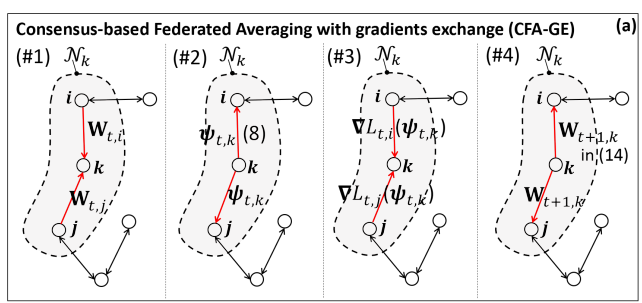
\includegraphics[scale=0.55]{Pic33.png}
			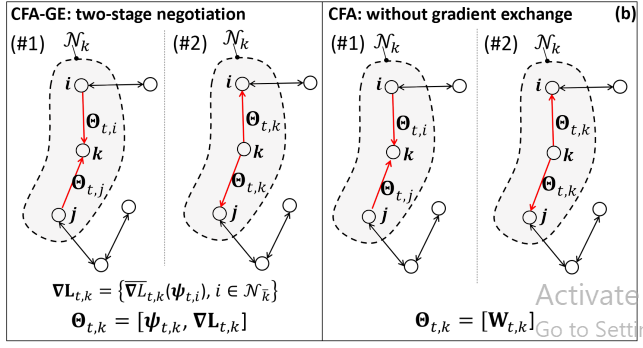
\includegraphics[scale=0.55]{Pic35.png}
		\caption{مراحل تبادل گرادیان‌ها و به‌روزرسانی مدل در الگوریتم \lr{CFA-GE}\cite{Fed11}}
		\label{Pic33}
	\end{center}
\end{figure}

مرحله اول آن مشابه الگوریتم \lr{CFA} است و $\phi_{t,k}$ را با تجمیع مدل مبتنی بر اجماع بدست می‌آورد. قبل از استفاده از $\phi_{t,k}$ برای به‌روزرسانی مدل محلی، به همان همسایگان بازخورد داده می‌شود (مرحله "مذاکره" یا \lr{negotiation} در مرحله 2 شکل \ref{Pic33}). سپس مدل $\phi_{t,k}$ توسط همسایگان برای محاسبه گرادیان‌ها با استفاده از داده‌های محلی آنها استفاده می‌شود. توجه داشته باشید که همه گرادیان‌ها بر روی یک دسته (یا مینی دسته) از داده‌های محلی محاسبه می‌شوند، در حالی که دسته/مینی‌دسته انتخابی می‌تواند در دورهای ارتباطی متوالی تغییر کند. گرادیان‌ها به دستگاه $k$ در مرحله 3 برمی‌گردند. در مقایسه با \lr{CFA}، این مرحله به هر دستگاهی اجازه می‌دهد تا با استفاده از داده‌های همسایه از گرادیان‌های اضافی بهره‌برداری کند و یادگیری را بسیار سریع‌تر می‌کند. بنابراین در دستگاه $k$، مدل محلی با استفاده از گرادیان‌های دریافتی $\nabla L_{t,k}(\phi_{t,k})$ مطابق رابطه \ref{e129} به‌روزرسانی می‌شود.

\begin{equation}\label{e129}
	\phi_{t,k}=\phi_{t,k}-\eta_t \sum_{i\in N_k}\beta_{k,i}P_{\Theta}[\nabla L_{t,i}(\phi_{t,k})]
\end{equation}
که $\beta_{k,i}$ وزن‌های ترکیب برای گرادیان‌ها هستند. در نهایت، همانطور که برای \lr{CFA} انجام شد.، به‌روزرسانی گرادیان با استفاده از مدل تجمیع‌شده $\phi_{t,k}$ و دسته دادهای محلی انجام می‌شود.

\begin{equation}\label{e130}
	w_{t+1,k}=\phi_{t,k}-\eta_t \nabla L_{t,k}(\phi_{t,k})
\end{equation}
برخلاف \lr{CFA}، \lr{، CFA-GE} نیاز دارد از پهنای باند و دورهای ارتباطی بیشتر برای تبادل همزمان گرادیان‌ها استفاده کند. به طور خاص، به استفاده فشرده‌تر از پیوندهای بی‌سیم \lr{D2D} برای به اشتراک‌گذاری مدل‌ها ابتدا در طول مذاکرات (مرحله شماره 2) و سپس ارسال گرادیان‌ها (مرحله 3) نیاز دارد. علاوه‌براین، هر دستگاه باید قبل از اعمال هر به‌روزرسانی مدل منتظر شیب‌های همسایه باشد. پیاده‌سازی دو مرحله‌ای \lr{CFA-GE}، اجرای روش مذاکره را برای بهبود زمان همگرایی (و تأخیر) ساده می‌کند. به عبارتی، هر دستگاه می‌تواند به‌روزرسانی‌ها را بدون انتظار برای پاسخ از همسایگان انجام دهد. با یک تعمیم ساده، دستگاه \lr{k} پارامترها را با همسایگان در دوره $t$ به صورت زیر مبادله می‌کند:
\begin{equation}\label{e130}
	\Theta_{t,k}=[\Phi_{t,k},\nabla L_{t,k}], \qquad  \nabla L_{t,k}:=\{\overline{\nabla L}_{t,k}(\phi_{t-1,i}),\forall i\in N_k\}	
\end{equation}

در راستای تکنیک‌های مبتنی بر تکانه، برای پیش‌بینی‌های $\bar{\nabla L_{t,k}}$ از میانگین متحرک وزن‌دار نمایی چند متغیره گرادیان‌های گذشته استفاده می‌شود.
\begin{equation}\label{e131}
	\overline{\nabla L}_{t,k}(\phi_{t-1,i})=\varrho \nabla L_{t,k}(\phi_{t-1,i})+(1-\varrho)\overline{\nabla L}_{t-1,i}
\end{equation}

با فرض اینکه وسیله $k$ قادر باشد پیام‌های $\Theta_{t,i}=[\Psi_{t,i},\nabla L_{t,i}]$  
را از همسایگان در هر دور $t$ دریافت کند، گام تجمیع مدل و گام به‌روزرسانی مدل با استفاده از گرادیان‌های دریافتی به صورت زیر است:

\begin{equation}\label{e132}
	\phi_{t,k}=w_{t,k}+\epsilon_t \sum_{i\in N_k}\alpha_{k,i}(\phi_{t,i}-w_{t,k})
\end{equation}

\begin{equation}\label{e133}
	\overline{\phi}_{t,k}=\phi_{t,k}-\eta_t \sum_{i\in N_k}\beta_{k,i}P_\Theta[\overline{\nabla L}_{t,i}(\phi_{t-1,k})]
\end{equation}


در مقاله \cite{Fed7} رویکرد یادگیری غیرمتمرکز فدرال به نام \lr{C-FL}\footnote{\lr{Consensus-driven FL}} برای وسایل نقلیه خودکار متصل به منظور دسته‌بندی عوامل جاده ارائه شده است. عوامل جاده مانند عابران پیاده، مخروط‌های ترافیکی، موانع، دوچرخه‌ها، اتومبیل‌ها و اتوبوس‌ها  که هر وسیله نقلیه آن‌ها را با اسکن محیط از طریق خود توسط سنسور \lr{Lidar} شناسایی می‌کند. نویسندگان یک روش سنجش مشارکتی را پیشنهاد کرده‌اند که در آن هدف وسایل نقلیه یادگیری مشارکتی یک مدل یادگیری ماشین عمیق مبتنی بر \lr{PointNet} برای استنباط نوع واقعی عوامل جاده با استفاده از ابرهای \lr{Lidar point } است. 

وسایل نقلیه مدل‌های محلی را با همسایگان‌شان از طریق اجماع میانگین ترکیب می‌کنند. سپس مدل‌های ترکیب شده با اجرای یک بهینه‌ساز روی داده‌های محلی خود به‌روزرسانی می‌کنند. فرایند یادگیری فدرال به طور کلی برای تعدادی دور ارتباطی اجرا می‌شود تا زمانی‌که یک اجماع حاصل گردد. در یادگیری فدرال پارامتر $w$ با اعمال یک روش کمینه‌سازی روی مجموع محدودی از توابع هدف یاد گرفته می‌شود.

\begin{equation}\label{e134}
	\hat{W}=\argminA_w L(w)=\argminA_w \sum_{i=1}^{N_\nu} \rho_i L_i(W)
\end{equation}
که $E_i=|\varepsilon_i|, \forall i\in\nu$ و $E=|\varepsilon|$ به ترتیب تعداد نمونه‌هاي وسیله نقلیه $i$ و تعداد کل نمونه‌های در دسترس است. $\rho_i=\frac{E_i}{E}$ است و $L_i(W)$ تابع خطا محلی وسیله نقلیه $i$ و $l(x_h,y_h;W)$ خطا محاسبه شده بر روی نمونه $(x_h,y_h)$ در حضور پارامترهای $W$ است. 
\begin{equation}\label{e135}
	L_i(w)=\frac{1}{E_i}\sum_{h=1}^{E_i}l(x_h,y_h;W)
\end{equation}
الگوریتم \lr{C-FL} یک زیرمجموعه بهینه‌سازی شده $W_{t,i}$ از لایه‌های مدل $Q<=N$ را هدف قرار می‌دهد، در حالیکه بقیه $N-Q$ فقط با استفاده از دادهای محلی و بهینه‌ساز انتخاب شده یادگرفته می‌شوند. برای $Q$ لایه پارامترهای مدل $W_{t,i}^{(Q)}$ بر روی هر دور ارتباطی تبادل می‌شوند. باقی لایه‌ها با استفاده از تنها داده‌های محلی یادگرفته می‌شوند و به صورت  $W_{t,i}^{(P)}=\{w_n^T,b_n\}_{n=1}^{N_Q-1}$ جمع آوری شده‌اند.

\begin{equation}\label{e136}
	W_{t,i}^{(Q)}=[w_{N-Q}^T,b_{N-Q},...,w_N^T,b_N]
\end{equation}
 
در هر دور ارتباطی وسیله نقلیه $i$ پارامترهای $Q$ لایه انتخاب شده و دریافت شده از همسایگانش  $j\in \nu_{t,i}$ را از طریق اجماع میانگین به‌روز می‌کند.
\begin{equation}\label{e136}
	\phi_{t,i}^{(Q)}=\sigma_{i,i}W_{t,i}^{(Q)}+\sum_{j\in \nu_{t,i}}\sigma_{i,j}W_{t,j}^{(Q)}
\end{equation}
که $\sigma_{i,j}$ وزن‌هایترکیب برای مدل‌های دریافت شده هستند و به صورت زیر مقداردهی می‌شوند:
\begin{equation}\label{e137}
\sigma_{i,j}=\frac{E_j}{\sum_{j\in \nu_{t,i}}E_j},\qquad \sigma_{i,i}=\frac{E_i}{\sum_{j\in \nu_{t,i}}E_j}
\end{equation}

به محض کامل شدن فرایند اجماع، وسیله نقلیه $i$ پارامترهای اشتراکی $\phi_{t,i}^{(Q)} $ با $W_{t,i}^{(P)} $ را به صورت $\phi_{t,i}=[W_{t,i}^{(P)}, \phi_{t,i}^{(Q)}]$ ترکیب کرده و بهینه‌ساز محلی را برای کمینه‌سازی خطای محلی $L_i(\phi_{t,i}^{(Q)})$ اجرا می‌کند. بهینه‌ساز \lr{Adam} به عنوان گزینه ترجیحی برای معماری‌های مبتنی بر \lr{PointNet} در نظر گرفته می‌شود که
\begin{equation}\label{e138}
W_{t+1,i}=\phi_{t,i}-\Delta \phi_{t,i}
\end{equation}

\begin{equation}\label{e139}
	\begin{cases}
		\Delta\phi_{t,i}=\eta_t\frac{\sqrt{1-\beta_2^T}}{1-\beta_1^t}\frac{m_{t+1,i}}{\sqrt{\nu_{t+1,i}}+\delta}\\
		m_{t+1,i}=\beta_1 m_{t,i}+(1-\beta_1)\nabla L_{t,i}(\phi_{t,i})\\
		\nu_{t+1,i}=\beta_2\nu_{t,i}+(1-\beta_2)\nabla^2 L_{t,i}(\phi_{t,i})
	\end{cases}
\end{equation}

که $m_{t+1,i}$ و $\nu_{t+1,i}$ تخمین‌های تکانه اول و دوم گرادیان‌های $\nabla L_{t,i}(\phi_{t,i})$ در دور $t+1$ هستند. پارامترهای جدید محاسبه شده $W_{t+1,i}$ به همسایگان وسیله نقلیه $i$ ارسال شده و دور جدید آغاز می‌شود. این فرایند تا زمانی‌که پارامترهای مدل به مقدار خطای موردنظر همگرا شوند، ادامه می‌یابد. 

\section{روش‌های موازی‌سازی‌ الگوریتم‌های توزیع‌شده و مدل‌های محاسباتی}
برای افزایش کیفیت پیش‌بینی‌ها و ارائه راه‌حل‌های یادگیری ماشین در مسائل پیچیده‌تر، مقدار قابل توجهی از داده‌های آموزش مورد نیاز است. اگرچه مدل‌های یادگیری ماشین کوچک را می‌توان با حجم کمی از داده مورد آموزش قرار داد، اما تعداد داده‌های آموزشی مورد نیاز مدل‌های بزرگتر همانند شبکه‌های عصبی با افزایش تعداد پارامترها، به طور تصاعدی رشد خواهد کرد و گاهی به راحتی به اندازه چندین ترابایت داده می‌رسند. هنگامی‌که داده‌ها ذاتاً توزیع‌شده یا داده‌ها برای ذخیره در یک ماشین واحد بسیار بزرگ باشند، راه‌حل‌های متمرکز گزینه مناسبی نمی‌باشند. به عنوان مثال می‌توان به پردازش معاملات در شرکت‌های بزرگ بر روی داده‌هایی که در مکان‌های مختلف ذخیره شده‌اند، اشاره کرد.

از آنجاکه تقاضا برای پردازش داده‌های آموزشی از افزایش قدرت محاسبات ماشین‌های محاسباتی سبقت گرفته است، نیاز به توزیع حجم داده‌ها یا حجم کار یادگیری در چندین ماشین احساس می‌شود و این امر موجب تبدیل سیستم متمرکز به یک سیستم توزیع‌شده خواهد شد و الگوریتم‌هایی باید انتخاب و اجرا شوند که محاسبات موازی، توزیع‌شدگی و مقاوم بودن در برابر خرابی‌ها را حمایت کنند. سیستم‌های توزیع‌شده چالش‌های جدیدی را ارائه می‌دهند که مهمترین چالش موازی‌سازی فرآیند آموزش و ایجاد یک مدل منسجم در این سیستم‌ها می‌باشد. 


در طراحي يك الگوريتم موازي بررسي ويژگي‌هايی همچون تسريع \footnote{\lr{Speedup}} و همگرايي الگوریتم بسيار حائز اهميت است \cite{nccl}. تسريع اصولا به صورت نسبت كل بار كاري انجام شده توسط يك گره به روي ميانگين بار كاري انجام شده توسط \lr{T} گره تعریف می‌شود. در کارهای تحقیقاتی اخیر، از تعاریف مختلفی برای مشخص کردن بار کاری جهت مقایسه کارآیی الگوریتم‌ها استفاده شده است. از جمله تعاریفی که برای تسریع در مقالات ارائه‌شده استفاده شده است، می‌توان به تسریع تکرار\footnote{\lr{Iteration speedup}} \ref{e15}، تسریع زمان اجرا \ref{e16}\footnote{\lr{Running time speedup}} و تسریع پیچیدگی \ref{e17} \footnote{\lr{Complexity speedup }} محاسباتی یا ارتباطی اشاره کرد. تسريع زمان اجرا، تسريع واقعي‌تری است اما از سخت‌افزار تاثير مي‌گيرد. تسريع تكرار كمتر تحت تاثير سخت افزار است و برای مقایسه الگوریتم‌های موازی معیار مناسب‌تری است \cite{lian2019}.

\begin{equation}\label{e15}
	Iteration speedup=\frac{number\ of\ iterations\ using\ one\ agent}{number\ of\ iterations\ using\ T\ agents}\times T
\end{equation}

پارامتر $T$ در رابطه تسریع تکرار  \ref{e15}  از میانگین‌گیری تعداد کل تکرارهای انجام شده توسط $T$ گره در مخرج حاصل شده است.
\begin{equation}\label{e16}
	Running time speedup=\frac{(running\  time\ using\ one\ agent)}{(running\ time\ of\ using\ T\ agents)}
\end{equation}

تسریع پیچیدگی زمانی نیز وابسته به سخت‌افزار نیست و می‌تواند انتخاب مناسبی برای ارزیابی و مقایسه الگوریتم‌های موازی‌ باشد. دلیل ظاهر شدن پارامتر $T$ در رابطه تسریع \ref{e17} همان است که برای رابطه \ref{e15} بیان شد.
\begin{equation}\label{e17}
	Complexity speedup=\frac{Complexity\ of\ the\ algorithm\ using\ one\ agent}{Complexity\  of\ using\ T\ agents}\times T
\end{equation}

علاوه‌بر ویژگی‌های مهم تسریع و نرخ همگرایی در طراحی الگوریتم‌های موازی، انتخاب پلتفرم مناسب برای پیاده‌سازی آن‌ها مبحث بسیار مهمی است و بر کارآیی الگوریتم تاثیر خواهد داشت. پياده‌سازي الگوريتم‌هاي موازي بر روي پلتفرم‌هاي 1) سیستم حافظه توزیع‌شده یا شبكه كامپيوتري 2) سيستم حافظه اشتراكي (\lr{multi-core } يا \lr{many-core}) قابل اجرا است\cite{lian2019}. در پردازنده‌های \lr{CPU} به دلیل داشتن کش‌های بزرگ، واحدهای‌ محاسبه و منطق قدرتمند و واحدکنترل بزرگ و پیچیده، مساله تاخیر تا حدی برطرف شده است  و اصطلاحا پردازنده‌های تاخیرگرا\footnote{\lr{Latency-oriented processors}} نامیده می‌شوند. پردازنده‌های \lr{GPU} به دلیل داشتن کش‌های کوچک، هسته‌های بسیار زیاد و امکان \lr{pipline} بالا، سرعت هسته‌ها بالاتر است و بازدهی عملیات افزایش می‌یابد و اصطلاحا پردازنده‌های نرخ‌گرا\footnote{\lr{Throughput-oriented processors}} نامیده می‌شوند. عملیاتی که در \lr{CPU}ها قابل اجرا هستند، به دلیل واحد کنترل بزرگ، متنوع‌تر خواهند بود. در صورتی‌که عملیات انجام‌شده در هسته‌های پردازنده \lr{GPU} خیلی سبک و در حد اجرا بر روی نخ‌ها\footnote{\lr{Thread}}  می‌باشند \cite{Kirk2017, So2015}.

در الگوریتم‌های موازی مبتنی بر شبکه کامپیوتری به دلیل بهره‌مندی هر گرهس از حافظه محلی و داشتن یک کپی از بردار مدل یا پارامتر در حافظه محلی خودش، خواندن و نوشتن بر روي كل بردار پارامتر به صورت اتميك امکان‌پذیر است اما در الگوریتم‌های موازی‌شده مبتنی بر سیستم‌های حافظه اشتراکی به دلیل استفاده تمام گره‌ها از یک حافظه مشترک که بردار مدل یا پارامتر بر روی آن ذخیره شده است، عملیات خواندن و نوشتن بر روي يك جز از بردار پارامتر به صورت اتميك قابل اجرا است \cite{GerBook}.
%--------------------------------------------------------------------
\subsection{الگوریتم‌های گرادیان کاهشی توزیع‌شده}

الگوریتم گرادیان کاهشی تصادفی\footnote{\lr{Stochastic Gradient Decent}} (\lr{SGD}) روشی مبتنی بر تکرار برای بهینه‌سازی یک تابع مشتق‌پذیر یا همان تابع هدف است که یک تقریب تصادفی از روش گرادیان کاهشی می‌باشد. در حقیقت گرادیان کاهشی تصادفی طی چند حلقه تکرار مقدار کمینه تابع هدف و مقادیری را که بازای آن‌ها تابع مقدار کمینه خود را می‌گیرد، بدست می‌آورد \cite{Zha2004}. تفاوت گرادیان کاهشی تصادفی با گرادیان کاهشی استاندارد\footnote{\lr{Gradient Decent}} (\lr{GD}) در این است که در گرادیان کاهشی استاندارد برای بهینه‌سازی تابع هدف از تمام داده‌های آموزشی استفاده می‌شود، در حالی‌که در گرادیان کاهشی تصادفی برای بهینه‌سازی تابع هدف از یک نمونه یا دسته‌ای از داده‌های آموزشی تصادفی استفاده می‌شود. این روش در مسائل آماری و یادگیری ماشین کاربرد فراوانی دارد \ref{hu2018}. در ادامه نوشتار به طور خلاصه چند نکته اساسی و مهم از الگوریتم‌های \lr{SGD} و \lr{GD} لیست شده است.

\begin{itemize}
	\item 
	در \lr{SGD}، قبل از حلقه تکرار باید نمونه‌های آموزشی به صورت تصادفی بُرزده\footnote{\lr{shuffling}} شوند.
	\item 
	در \lr{SGD}، به دلیل اینکه در هر لحظه تنها یک نمونه یا یک دسته‌ای از نمونه‌ها استفاده می‌شود، مسیر همگرایی آن تصادفی‌تر از \lr{GD} است. اما تا زمانیکه حداقل زمان آموزش را به ما بدهد این مسیر بی‌اهمیت است.
	\item 
	به الگوریتم‌هایی که در هر تکرار به جای یک نمونه داده \lr{n } نمونه (یا یک دسته) استفاده می‌کنند، الگوریتم‌های  \lr{Mini-batch GD } می‌گویند.
\end{itemize}	


با توجه به ماهیت ترتیبی بودن الگوریتم \lr{SGD} مقیاس‌پذیری آن محدود بوده و در نتیجه موازی‌سازی آن دشوار است \cite{Hog12011}. با این وجود، با عرضه پردازنده‌های ارزان قیمت چندهسته‌ای و حجم بالای داده‌ها در مقیاس وب، محققان را بر آن داشته است تا چندین طرح موازی‌سازی هوشمندانه برای \lr{SGD} ارائه دهند. از آنجایی‌که بسیاری از مجموعه‌ داده‌های بزرگ در یک چارچوب پردازش موازی مانند \lr{MapReduce} از پیش‌ پردازش شده‌اند، بیشتر کارهای انجام‌شده اخیر بر روی \lr{SGD} موازی بر پیاده‌سازی \lr{MapReduce} متمرکز شده‌اند. همان طور که قبلا هم اشاره شده است، \lr{MapReduce} ابزاری قدرتمند در گوگل است که برای استخراج اطلاعات از لاگ‌های بسیار بزرگ و اطمینان از تحمل خطا و ساده‌سازی تعمیر و نگهداری و برنامه‌نویسی کلاسترهای بزرگ طراحی شده است \cite{Gem2011}. اما به طور ایده‌آل این روش برای تجزیه و تحلیل داده‌های برخط و عددی فشرده مناسب نیست. همچنین بیان محاسبات تکرارشونده در آن دشوار است و هزینه بالای آن برای اطمینان از تحمل خطا می‌تواند منجر به کارآیی نامطلوب شود. در واقع، حتی محققان گوگل نیز بیان می‌کنند که سیستم‌های دیگر برای کارهای تجزیه و تحلیل داده‌ها مناسب‌تر از \lr{MapReduce} هستند.  
 
 سیستم‌های چندهسته‌ای دارای مزایای قابل توجهی هستند، از جمله (1) تأخیر کم و حافظه اصلی مشترک با توان عملیاتی بالا؛ و (2) پهنای باند بالای چندین دیسک. در مقابل \lr{MapReduce} به دلیل بررسی‌های مکرر برای تحمل خطا، داده‌های دریافتی را با نرخ کمتری می‌خواند. با توجه به نرخ‌ بالای سیستم‌های چندهسته‌ای، چالش مطرح در محاسبات موازی این نوع سیستم‌ها موضوع همگام‌سازی (یا قفل کردن) پردازنده‌ها خواهد بود. بنابراین برای فعال‌کردن تجزیه و تحلیل داده‌های مقیاس‌پذیر بر روی یک سیستم چندهسته‌ای، هر طرح موازی باید به گونه‌ای باشد که نیاز به قفل اضافی و همگام‌سازی بین پردازنده‌ها را به حداقل برساند \cite{ag2011}. اخیراً طرح‌های متعددی برای موازی‌سازی الگوریتم \lr{SGD} پیشنهاد شده است، اكثر طرح‌های مطرح‌شده نیاز به همگام‌سازي گره‌ها و يا قفل‌کردن برای کنترل دسترسی همزمان گره‌ها به حافظه اشتراکی دارند. این موارد سبب پایین آمدن کارایی طرح‌های موازی مي‌شود. با توجه به اینکه قفل‌های نرم‌افزاری هزینه‌های بسیار زیادی دارند، در حالت ایده‌آل طرحی مناسب است که بدون انتظار\footnote{\lr{Wait-Free}} و بدون قفل\footnote{\lr{Lock-Free}} باشد.
 
 در این بخش به بررسی و مقایسه کارهای ارائه شده در حوزه یادگیری توزیع‌شده مبتنی بر الگوریتم گرادیان کاهشی پرداخته می‌شود. تمرکز این کارها بیشتر بر روی مباحثی همچون نحوه توزیع داده‌ها و مدل بین گره‌ها (به عبارت دیگر استفاده از روش‌های داده-موازی و مدل-موازی)، یادگیری توزیع‌شده متمرکز مبتنی بر سرور پارامتر و یادگیر غیرمتمرکز بدون حضور سرور مرکزی، نحوه برخورد با محیط‌های محاسباتی ناهمگن در الگوریتم‌های یادگیری توزیع‌شده، پلتفرم موازی حافظه اشتراکی یا حافظه توزیع‌شده و روش‌های همگام‌سازی بین گره‌ها، می‌باشد.
 
 یک استراتژی ساده برای اجرای \lr{SGD} به صورت موازی و بدون قفل به نام \lr{Hogwild! } در مقاله \cite{Hog12011} ارائه شده است که پردازنده‌ها (گره‌ها) اجازه دسترسی یکسان به حافظه اشتراکی را دارند و می‌توانند اجزای مجزای حافظه را به دلخواه خود به‌روزرسانی کنند. از آنجایی که پردازنده‌ها می‌توانند تغییرات پردازنده‌های دیگر را بازنویسی کنند، الگوریتم بدون قفل ممکن است دچار مشکل شود. در این مقاله نشان داده شده است که وقتی دسترسی به داده‌ها به صورت خلوت  باشد (به عبارتی گام‌های مجزا \lr{SGD} فقط بخش کوچکی از بردار پارامتر را به‌روزرسانی می‌کنند) بازنویسی حافظه توسط پردازنده‌های مختلف به ندرت رخ می‌دهد و در صورت بروز در محاسبات خطا دیده خواهد شد. در این استراتژی یک تسریع تقریبا خطی با توجه به تعداد پردازنده‌ها برای مسائل یادگیری خلوت از نظر تئوری و تجربی ارائه شده است اما همان طور که بیان شد تنها برای مسائل بهينه‌سازي خلوت قابل اعمال است. تابع هزینه خلوت در استراتژی \lr{Hogwild!} به صورت زیر تعریف می‌شود:
 
 \begin{equation}\label{e18}
 	f(w)=\sum_{e\in E}f_e(w)
 \end{equation}
 
 که بردار پارامتر $w$ در حافظه اشتراكي ذخيره می‌شود و توسط تمام پردازنده‌ها در دسترس است. $e$ زیرمجموعه کوچکی از $\{1, 2, ...,M\}$ است و $x_e$ مقادير بردار $w$ با توجه به نقاط انتخاب شده در $e$ را نشان می‌دهد. 
 \begin{equation}\label{e19}
 	|E|^{-1}G_e(x_e)\in \partial f_e(w)
 \end{equation}
 
 در مقاله \cite{Zin2010} یک الگوریتم \lr{SGD} موازی بر اساس یک استراتژی تک-میانگین‌گیری  به نام \lr{SimuParallel SGD } ارائه شده است و مبنا را بر مدل موازی‌سازی داده گذاشته است. به عبارتی \lr{m } نمونه داده بین \lr{k} پردازنده تقسیم شده و در هر تکرار $t$ هر پردازنده \lr{i} به صورت مستقل و بدون هیچ تبادل و همکاری با دیگر پردازنده‌ها، گرادیان کاهشی تصادفی را با توجه به داده‌ $c^{i,t}$ و بردار پارامتر $w_{i,t}$ محاسبه می‌کند. زمانی که اجرای تمام پردازنده‌ها به پایان رسید، در نقطه همگام‌سازی نتایج تجمیع و سپس میانگین آنها به عنوان نتیجه نهایی در نظر گرفته می‌شود.
 
در صورتی‌که گره‌های شرکت‌کننده در فرایند یادگیری توزیع‌شده از لحاظ قدرت محاسباتی و پردازشی با یکدیگر متفاوت باشند، پردازنده‌ها با عملکرد پایین تاثیر منفی بر نتیجه نهایی خواهند گذاشت. در \cite{WP2020} یک الگوریتم گرادیان کاهشی موازی وزن‌دار به نام \lr{WP-SGD } معرفی شده است که بردارهای پارامتر گره‌ها به صورت وزن‌دار برای تولید نتیجه نهایی با یکدیگر ترکیب می‌شوند. وزن اختصاص داده شده به بردار پارامتر هر گره بر اساس تاخیر بین آن و سریع‌ترین گره تعریف شده است.
 
 الگوریتم گرادیان کاهشی تصادفی موازی همزمان\footnote{\lr{Synchronous Parallel Stochastic Gradient Descent (S-PSGD)}}  \lr{(S-PSGD)} یک روش یادگیری توزیع‌شده موازی است که در مقاله \cite{Mini2016} برای حل توابع هزینه غیرمحدب و در \cite{dekel2012} برای حل توابع هزینه محدب معرفی شده است. پیاده‌سازی این الگوریتم به صورت متمرکز و با حضور یک سرور پارامتر  \footnote{\lr{Parameter server}} انجام شده است. در هر گام هر گره بردار پارامتر را از سرور پارامتر خوانده و گرادیان تصادفی دسته‌ای را محاسبه می‌کند. سپس گره‌ها گرادیان‌های خود را به سرور پارامتر ارسال کرده و بعد از همگام‌سازی، با استفاده از میانگین گرادیان‌ها بردار پارامتر ذخیره‌شده در سرور پارامتر به‌روزرسانی می‌شود. به دلیل وجود گام همگام‌سازی، اکثر گره‌ها باید در حالت انتظار قرار بگیرند تا کار آهسته‌ترین گره به اتمام برسد. در این روش هزینه گام‌ همگام‌سازی $O(N)$ است. زمانی که $N$ بزرگ باشد، سبب هزینه‌های ارتباطی بالا در سرور پارامتر می‌شود. 
 
 در مقاله \cite{nccl} برای پیاده‌سازی الگوریتم \lr{AllReduce-SGD } از قانون به روزرسانی‌ای دقیقاً مشابه \lr{S-PSGD} در هر تکرار استفاده شده است. هیچ سرور پارامتری در این الگوریتم وجود ندارد. گره‌ها با یک شبکه حلقه بهم متصل شده‌اند و هر گره نسخه محلی از مدل را نگه می‌دارد. در هر تکرار، هر گره گرادیان دسته‌ای را محاسبه کرده و سپس از \lr{AllReduce} برای همگام‌سازی گرادیان‌ها استفاده می‌کنند. در نهایت هر گره میانگین همه گرادیان‌ها را بدست می‌آورد. این الگوریتم در شبکه‌ای با تاخیر بالا کند عمل خواهد کرد. در پایان تکرار، مدل محلی هر گره با میانگین گرادیان‌ها به‌روز می‌شود. به دلیل وجود همگام‌سازی در هر تکرار، زمان بیکاری همانند الگوریتم \lr{S-PSGD} بالا است. 
 
در یک محیط ناهمگن\footnote{\lr{Heterogeneous environment}}  که گره‌ها از لحاظ قدرت محاسباتی و ارتباطی متفاوت هستند، الگوریتم‌های همزمان عملکرد ضعیفی دارند. از طرفی، الگوریتم‌های غیرهمزمان که با استفاده از یک سرور پارامتر پیاده‌سازی می‌شوند از مشکلاتی همانند: 1) گلوگاه ارتباطی در سرورهای پارامتر با تعداد گره‌های زياد 2) كاهش ميزان همگرايي با متراكم شدن ترافيك سرور پارامتر، رنج می‌برند. 
 
 ماشین‌های  \lr{NUMA}\footnote{\lr{Non-Uniform Memory Access}} از تعدادی پردازنده \lr{CPU} با هسته‌های زیاد تشکیل شده‌اند. به عبارت دیگر مدلی از طراحی سخت‌افزاری است که در سرورهایی با چند \lr{CPU} استفاده می‌شود و استفاده از حافظه توسط یک پردازنده \lr{CPU} کاملا بستگی به مکان قرار گرفتن حافظه نسبت به آن دارد. استراتژی  \lr{DimmWitted} \cite{DimmWitted} یک تحلیل آماری بر روی روش‌های تکثیر مدل و داده و همچنین شیوه‌های دسترسی به داده‌ها در حافظه اصلی يك ماشين \lr{NUMA} ارائه داده است. در واقع گره‌ها بر روی گره‌های یک ماشین \lr{NUMA} پیاده‌سازی شده‌اند و همگام‌سازي مدل‌ها بر روي گره‌ها انجام می‌شود. این همگام‌سازی تا زمانی‌ که مانع عبور و مرور داده‌ها در حافظه اصلی نشود، سودمند است. به منظور همگام‌سازی در این استراتژی، یک نخ در هر گره به صورت متناوب مدل‌های روی تمام گره‌ها را می‌خواند و پس از میانگین‌گیری نتایج، کپی مدل ‌در گره را به‌روزرسانی می‌‌کند.
 
در مقاله \cite{lian2019} با استفاده از دو پلتفرم حافظه اشتراکی و شبکه کامپیوتری (حافظه توزیع‌شده) دو الگوریتم \lr{SGD} توزیع‌شده موازی غیرهمزمان\footnote{\lr{Asynchronous}} به صورت متمرکز برای حل مسائل بهینه‌سازی غیرمحدب معرفی شده است. این الگوریتم با نام \lr{A-PSGD } شناخته شده‌است که در مقاله \cite{ag2011} از این الگوریتم برای حل مسائل محدب نیز استفاده شده است. در الگوریتم \lr{AsySG-con} \cite{lian2019} که بر روی پلتفرم شبکه‌ کامپیوتری پیاده‌سازی شده است، بردار پارامترها بر روی سرور مرکزی قرار دارد و در طول گام به‌روزرسانی، گره‌ها اجازه دسترسی به بردار پارمترها را ندارند. در نتیجه فرآیند خواندن بردار سازگار خواهد بود. برای ایجاد ارتباط بین گره‌ها و سرور مرکزی از کتابخانه \lr{MPICH} کمک گرفته شده است. برای پياده‌سازي الگوریتم‌های غيرهمزمان، از یک پارامتر کهنگی\footnote{\lr{Staleness}}  استفاده می‌شود و مقادير قديمي بردار پارامتر براي ارزيابي گراديان تصادفي سایر گره‌ها به‌کار گرفته می‌شود. هر گره داده‌های نمونه را به صورت دسته‌های \lr{M}تایی تصادفی دریافت کرده و پس از محاسبه گرادیان آن را به سرور مرکزی ارسال می‌کند. سرور مرکزی با قبول یک میزان کهنگی $\tau _{k,m}$ در پارامترهای دریافتی از گره‌های شبکه به‌روزرسانی بردار پارامتر $w_{k+1}$ را انجام می‌دهد. 
 
 \begin{equation}\label{e23}
 	w_{k+1}=w_k-{\gamma}_k \sum_{m=1}^{M}G(x_{k-\tau_{k,m}},\xi_{k,m})
 \end{equation}
 
 میزان کهنگی گرادیان‌های دریافتی از گره نباید از یک حدی بیشتر باشد. زیرا همگرایی الگوریتم را به شدت کاهش می‌دهد و در بعضی مواقع سبب واگرایی آن می‌شود. براي داشتن همگرايي مناسب، میزان کهنگی نبايد زياد بزرگ باشد و یک حدآستانه‌ به صورت $\max_{k,m} \tau _{k,m}\le T$ در نظرگرفته شود \cite{Avron2014}.
 
در الگوریتم \lr{AsySG-INcon} \cite{lian2019} که بر روی پلتفرم حافظه اشتراکی پیاده‌سازی شده است، بردار پارامتر \lr{w} بر روی حافظه اشتراکی قرار می‌گیرد و هر گره بردار پارامتر را از حافظه خوانده و در حافظه محلی خود قرار می‌دهد و با استفاده از داده‌های نمونه و $\hat{w ̂}$ (مقدار خوانده شده از حافظه اشتراکی)  مقدار گرادیان $G(\hat{w}_k;\xi_k)$ را به صورت محلی محاسبه می‌کند. سپس بردار پارامتر $w$ در حافظه اشتراکی بدون قفل نرم‌افزاری به صورت زیر به‌روزرسانی می‌شود.
 \begin{equation}\label{e24}
 	(w_{k+1})_{i_k}=(w_k)_{i_k}-\gamma \sum_{m=1}^{M}(G(\hat{w}_{k,m},\xi_{k,m}))_{i_k} 
 \end{equation}
 
 که $i_k\in \{{1,2,…,M}\}$ یک اندیس تصادفی انتخاب شده برای به‌روزرسانی توسط گره \lr{k} و \lr{n} طول بردار پارامتر را نشان می‌دهد. الگوریتم \lr{A-PSGD } بر روی حافظه اشتراکی از مشکل خواندن‌های ناسازگار رنج می‌برد. راه‌حل استفاده شده برای غلبه بر این مشکل برگرفته از روش ارائه شده در \cite{Avron2014} می‌باشد. با مانیتور کردن مقدار بردار پارامتر در حافظه اشتراکی و استفاده از تعریف  $w_k$ به صورت زیر تا حدی این مشکل را می‌توان برطرف کرد:
 \begin{equation}\label{e25}
 	\hat{w}_k=w_k-\sum_{j\in J(k)} (w_{j+1}-w_j) 
 \end{equation}
 
 \begin{equation}\label{e26}
 	J(k)\subset {k-1,...,k-T}, \quad \lvert J(k)\rvert\le T
 \end{equation}
 
 مجموعه $J(k)$ در رابطه \ref{e26} برای مانیتور کردن مقدار بردار پارامتر  در حداکثر $T$ گره دیگر است. 
 
 زمانی‌که شرایط شبکه مساعد باشد، روش‌های \lr{SGD} موازی توزیع‌شده تسریع مشابه‌ای خواهند داشت و تفاوت این روش‌ها زمانی مشخص می‌شود که شبکه‌ای با پهنای باند کم و در نتیجه تاخیر بالا داشته باشیم. در الگوریتم \lr{D-PSGD} \cite{Lian20171} با حذف سرور مرکز سعی شده است یک \lr{SGD} موازی غیرمتمرکز همزمان برای کاهش بار ترافیکی سرور و برطرف کردن معایب الگوریتم‌های قبلی معرفی شود. یکی از معایب این الگوریتم هزینه بالای همگام‌سازی گره‌ها در شبکه است. برای توزیع دادها می‌توان کل داده‌ها را در اختیار همه گره‌ها قرار داد یا داده‌ها را به شکلی مناسب پارتیشن‌بندی کرد و هر پارتیشن را در اختیار یک گره قرار داد. برای پیاده‌سازی این الگوریتم از چارچوب‌کاری یادگیری عمیق ماکروسافت \lr{CNTK} و کتابخانه \lr{Torch} استفاده شده است. 
 
 در مقاله \cite{lian2018} الگوریتم غیرمتمرکز غیرهمزمان  \lr{AD-PSGD } برای یادگیری موازی توزیع‌شده معرفی شده و معایب رویکردهای قبلی را برطرف کرده است. برای هر گره \lr{i} یک نخ محاسباتی (برای انجام محاسبات گرادیان‌ها و به‌روزرسانی وزن‌ها) و یک نخ ارتباطی (برای برقرار ارتباط بین گره \lr{i} و یک همسایه تصادفی و ترکیب بردار وزن‌ آنها) با یک بافر مشترک \lr{g} تعریف شده است که به ترتیب بر روی \lr{GPU} و \lr{CPU} اجرا می‌شوند. پردازنده‌های \lr{GPU} به طور پيوسته گراديان‌ها را محاسبه و نتايج را بدون توجه به اينكه ميانگين‌گيري رخ مي‌دهد يا خير، در بافر پردازنده‌های \lr{CPU} قرار مي‌دهند. در این مقاله گره‌ها به دو دسته فعال و غیرفعال تقسیم می‌شوند. به منظور جلوگیری از بن‌بست در تبادل و میانگین‌گیری بردارهای پارامتر دو گره انتخاب‌ می‌شود، به طوریکه یک گره فعال همسایه‌اش را تنها از مجموعه گره‌های غیرفعال می‌تواند انتخاب کند. به منظور مدیریت فرآیند یادگیری غیرهمزمان از یک تکنیک کهنگی استفاده شده است. 
 
 رویکرد‌های موازی و توزیع‌شده‌ای که اخیرا مبتنی بر الگوریتم گرادیان کاهشی ارائه شده‌اند، از لحاظ ویژگی‌هایی مانند نرخ همگرایی، پیچیدگی ارتباطی، زمان بی‌کاری یا معطلی و پلتفرم موازی استفاده‌شده در شکل \ref{p31} لیست شده‌اند. معیار پیچیدگی ارتباطی در جدول بر اساس نسبت $\frac{n_t}{n_h}$ تعریف شده است. که $n_t$ تعداد گرادیان‌ها یا مدل‌های انتقال‌داده‌ شده در پرمشغله‌ترین گره در هر \lr{n} به‌روزرسانی گرادیان تصادفی و $n_h$ تعداد دست‌تکان‌دادن‌های انجام‌شده در پرمشغله‌ترین گره در هر \lr{n} به‌روزرسانی گرادیان تصادفی را نشان می‌دهند. 
 \begin{figure}[h]
 	\begin{center}
 		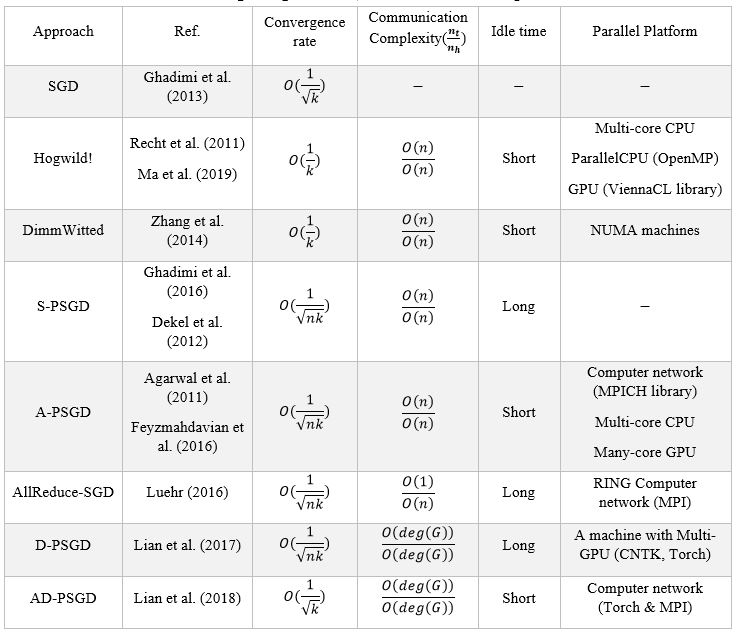
\includegraphics[scale=1.2]{Pic31.JPG}
 		\caption{جمع‌بندی الگوریتم‌های موازی \lr{SGD} و برخی از ویژگی‌های مورد نظر آن‌ها}
 		\label{p31}
 	\end{center}
 \end{figure}
 
 در مقاله \cite{Ma2019} دو روش موازی‌سازی \lr{SGD} همزمان و \lr{SGD} غیرهمزمان با استفاده از معماری‌های‌ محاسباتی مختلف در یک سیستم واحد پیاده‌سازی شدند و تاثير آنها بر روي كارايي سخت افزاري و زمان همگرايي در حالت‌هاي مختلف داده و توابع زیان متفاوت مورد بررسي قرار گرفته است. آن‌ها به این نتیجه دست یافتن که انتخاب بين نوع معماری محاسباتی و روش به‌روزرسانی مدل  به نوع کار و ويژگي داده‌ها وابسته است. در روش \lr{SGD} همزمان، يك نخ مسئول به‌روزرساني مدل است. اين روش سبب محدود شدن اجراي موازي داخل الگوریتم مي‌شود. بهترین انتخاب برای موازی‌سازی عبارت جبرخطي، گراديان تابع زیان در مرحله محاسبه گراديان می‌باشد که براي تسريع محاسبات، پياده‌سازي‌هاي موازي كارا از كتابخانه‌هاي جبرخطي بهينه‌شده همچون کتابخانه \lr{ViennaCL} استفاده مي‌شود. این کتابخانه هم برای داده‌های خلوت و هم داده‌های متراکم کاربرد دارد. در صورتی‌که کتابخانه تنسورفلو و دیگر چهارچوب‌های کاری یادگیری عمیق تنها داده‌های متراکم را پشتیبانی می‌کنند و نمی‌توانند مدل‌های با ابعاد خیلی بالا را مدیریت کنند. 
 
 یک الگوریتم \lr{SGD} توزیع‌شده بر اساس روش‌های بُرزدن محلی\footnote{\lr{Local shuffling}}  و سراسری\footnote{\lr{Global shuffling}}  با استفاده از یک گره مرکزی در مقاله \cite{MENG201946} ارائه شده است. بُرزدن یکی از روش‌های رایج پردازش داده است که برای حل مسائل بزرگ یادگیری ماشین از تقسیم‌بندی داده‌ها در طول چندین ماشین یا نخ کاربرد دارد. در الگوریتم ارائه شده، داده‌های آموزشی برزده می‌شوند و سپس داده‌ها به صورت زیرمجموعه‌های غیرهمپوشان تقسیم شده و هر زیرمجموعه به یک گره اختصاص می‌یابد. بعد از انجام فرآیند یادگیری در هر تکرار، مجددا بُرزدن به صورت محلی یا سراسری انجام می‌شود. اگر بُرزدن به صورت سراسری باشد، بعد از بُرزدن داده‌ها مجدد در هر تکرار تقسیم‌بندی داده‌های آموزشی به صورت زیرمجموعه‌های غیرهمپوشان انجام می‌شود اما اگر بُرزدن به صورت محلی انجام شود، دیگر نیازی به تقسیم‌بندی مجدد داده‌های آموزشی نیست. نویسندگان مقاله نشان دادند که اگر عملیات بُرزدن مستقل باشد، بُرزدن سراسری معادل نمونه‌گیری بدون جایگزینی است و آن‌ها همگرایی الگوریتم \lr{SGD} توزیع‌شده به روش بُرزدن محلی و سراسری را برای مسائل غیرمحدب اثبات کردند. نرخ همگرایی برای بُرزدن محلی کندتر از بُرزدن سراسری است، زیرا اگر ارتباطی بین داده‌های تقسیم شده وجود نداشته باشد، برخی اطلاعات را از دست خواهیم داد.
 
 از آنجایی که قدرت محاسباتی گره‌های شبکه ممکن است متفاوت باشد، با هدف افزایش نرخ همگرایی و استفاده بهینه از منابع در دسترس به طور همزمان، در مقاله \cite{Ma2021} یک الگوریتم‌ \lr{SGD} توزیع‌شده با اندازه‌‌ دسته داده‌های سازگار  مبتنی بر معماری‌های ناهمگن \lr{CPU+GPU}  پیشنهاد شده است. میزان داده‌های اختصاص‌یافته به هر گره توسط یک گره هماهنگ‌کننده \footnote{\lr{Coordinator node}} به صورت پویا و تطبیقی در زمان اجرا و براساس سرعت پردازش آن گره تعیین می‌شود. 
 
 در یک کار متفاوت \cite{Pu2021}، مساله بهینه‌سازی توزیع‌شده بر روی گراف‌های متغیر با زمان در نظر گرفته‌ شده است و یک الگوریتم ردیابی گرادیان تصادفی توزیع‌شده (\lr{DSGT})\footnote{\lr{Distributed stochastic gradient tracking algorithm}}  با معرفی متغییر کمکی $y_i$  برای هر گره به منظور ردیابی میانگین گرادیان تصادفی توابع هزینه را با فرض در دسترس بودن اطلاعات گرادیان دقیق، ارائه شده‌ است. در مرجع \cite{time2017} نیز روشی مشابه ارائه شده است. روش دیگری در این مقاله  \cite{Pu2021} به نام ردیابی گرادیان تصادفی شایعه (\lr{GSGT})  پیشنهاد شده است که براساس پروتکل‌های ارتباطی مبتنی بر \lr{Gossip} بوده و برای کاهش هزینه‌های ارتباطی در محاسبات توزیع‌شده کاربرد دارد. در هر تکرار یک گره‌ $i_k\in k$ به صورت تصادفی با احتمال $\frac{1}{n}$ فعال شده و با یکی از همسایه‌های خود $j_k$ با احتمال $\pi_{i_k j_k}$ ارتباط برقرار می‌کند و یا با احتمال $\pi_{i_k i_k}=1-\sum_{j\in N_{i_k}}\pi_{i_k j_k}$  با خودش به‌روز می‌شود. گام به‌روزرسانی هر گره $i$ به صورت زیر می‌باشد:
 
 \begin{equation}\label{e27}
 	\begin{cases}
 		w_{i,k+1}=\frac{1}{2}(w_{i_k,k}+w_{j_k,k})-\alpha y_{i_k,k}\\
 		y_{i,k+1}=\frac{1}{2}(y_{i_k,k}+y_{j_k,k})+g_i(w_{i,k+1},\xi_{i,k+1})-g_i(w_{i,k},\xi_{i,k})
 	\end{cases}
 \end{equation}
 
 
\subsection{الگوریتم‌های توزیع‌شده مبتنی بر یک مدل محاسباتی موازی}

مدل‌های محاسباتی روش مفیدی برای هدایت طراحان الگوریتم‌های موازی و برنامه‌نویسان برای بهینه‌سازی کد و بهره‌برداری از ویژگی‌های سخت‌افزاری جدید است. همین طور که اشاره شد، در حوزه سیستم‌های یادگیری توزیع‌شده به منظور تسریع عملیات و مدیریت بهتر بخش‌های مختلف محاسبات و ارتباطات، پیاده‌سازی فرآیند یادگیری موازی توزیع‌شده باید تحت یک مدل محاسباتی موازی از جمله  \lr{PRAM}، \lr{LogP}، \lr{BSP} و \lr{MapReduce} انجام شود. مدل محاسباتی \lr{PRAM} یک مدل حافظه اشتراکی است و به دلیل محدودیت در تعداد پردازنده‌ها و بالا بودن هزینه ارتباطات نسبت به هزینه محاسبات برای پیاده‌سازی همه جانبه مناسب نیست. مدل محاسباتی \lr{LogP} مدل برنامه‌نویسی ندارد و ارتباطات پردازنده‌ها در آن به صورت یک نمای محلی بر اساس عملکرد هر جفت پردازنده است. در مقاله \cite{BSP2012} تفاوت‌های بین چارچوب نگاشت-کاهش و مدل محاسباتی \lr{BSP} مورد بحث قرار گرفته‌اند و این واقعیت برجسته شده است که الگوریتم‌های \lr{BSP} به دلیل نیاز به ذخیره‌سازی و دسترسی به داده‌ها در چندین ابرگام، در صورتی که تعداد ابرگام‌ها ثابت نباشد، نمی‌توانند به طور موثر با استفاده از چهارچوب نگاشت-کاهش پیاده‌سازی شوند. این مورد به دلیل ماهیت چارچوب نگاست-کاهش است که اجازه ذخیره‌سازی داده بین دورها را نمی‌دهد، اما الگوریتم‌های \lr{BSP} مستلزم این هستند که به این داده‌ها بین چنین دورهایی دسترسی داشته باشند. همچنین، آنها نشان دادند که مدل \lr{BSP} می‌تواند برای مدل‌سازی الگوریتم‌های نگاشت-کاهش با هزینه جانبی یکسان برای سیستم‌های معمولی با تعداد پردازنده‌های یکسان استفاده شود. بنابراین، مشخص شده است که \lr{MapReduce} باید صرفاً به عنوان یک چارچوب پیاده‌سازی با \lr{BSP} برای طراحی الگوریتم‌ها استفاده شود. با این حال، برای کارهایی با زمان اجرا ناشناخته، \lr{MapReduce} همچنان باید استفاده شود زیرا \lr{BSP} دارای قابلیت تعادل بار پویا نیست. به عنوان مثال، فریمورک محاسبات توزیع‌شده\lr{Apache hama } از مدل \lr{BSP} استفاده می‌کند و گره‌ها می‌توانند با یکدیگر ارتباط برقرار کنند، در حالیکه فریمورک \lr{Apache Hadoop} مبتنی بر چارچوب نگاشت-کاهش است و گره‌ها در انتهای هر دور تنها  مجاز به ارتباط با پردازنده مرکزی هستند. 

یکی از موضوعات مهم در طراحی سیستم‌های یادگیری توزیع‌شده \textbf{همگام‌سازی مانع}  یا \textbf{مکانیزم کنترل مانع} بین گره‌ها است. در حال حاضر، روش‌های کنترل مانع را می‌توان به طور کلی به سه مکانیزم موازی غیرهمزمان\footnote{\lr{Asynchronous Parallel}} (\lr{ASP})، مکانیزم موازی همزمان با کهنگی \footnote{\lr{Stale Synchronous Parallel}}(\lr{SSP}) و مکانیزم موازی همزمان مانعی\footnote{\lr{Bulk Synchronous Parallel}} (\lr{BSP}) دسته بندی کرد \cite{NIPS2012}. 

مکانیزم \lr{BSP} یک طرح قطعی است که در آن گره‌ها یک مرحله محاسباتی را انجام می‌دهند و به دنبال آن یک مرحله همگام‌سازی یا ارتباطات برای تبادل به‌روزرسانی‌ها را انجام می‌دهند. این روش اطمینان می‌دهد از طریق جلوگیری از رفتن هر گره به مرحله بعدی تا زمانی که همه گره‌ها بتوانند محاسبات را به اتمام برسانند، همه گره‌ها در یک تکرار محاسباتی یکسانی قرار خواهند داشت. علاوه بر این، اثرات محاسبات فعلی برای گره‌ها تا زمانی که مانع انجام نشده است، قابل مشاهده نیست. با توجه به اینکه تضمین‌های صحت برنامه سریال برای برنامه‌های \lr{BSP} اغلب قابل تحقق است، در نتیجه \lr{BSP} قوی‌ترین روش کنترل مانع خواهد بود \cite{Ho2013}. متأسفانه \lr{BSP} یک نقطه ضعف بزرگ دارد. از آنجایی که گره‌ها باید منتظر بمانند تا کار دیگران به پایان برسد، در صورت وجود گره‌هایی با قدرت محاسباتی کمتر در یک شبکه ناهمگن \cite{NIPS2012} و یا گره‌هایی که به دلیل عوامل تصادفی و غیرقابل پیش‌بینی به زمان بیشتری برای تکمیل یک مرحله نیاز دارند، کارایی محاسبات در این مدل براساس کندترین ماشین تعیین می‌گردد. این امر منجر به کاهش چشمگیر عملکرد سیستم می‌شود. به طور کلی، \lr{BSP} دقت محاسباتی بالایی دارد اما در محیط‌های ناهمگن از کارایی پایین رنج می‌برد.

مکانیزم \lr{ASP} ساده‌ترین مدل است که هیچ همگام‌سازی بین گره‌ها رخ نمی‌دهد. این مکانیزم نقطه متقابل مکانیزم کنترل مانع \lr{BSP} است و اجازه می‌دهد محاسبات با حداکثر سرعت ممکن از طریق اجرای کاملا غیرهمزمان گره‌ها انجام شوند. در محیط‌های محاسباتی همگن، که در آن گره‌ها پیکربندی‌ مشابهی دارند، مکانیزم \lr{ASP} هم‌گرایی سریعی دارد و بالاترین توان عملیاتی تکرار را نتیجه می‌دهد. اما در حالت کلی، این غیرهمزمانی باعث تاخیر در به‌روزرسانی و اعمال نویز و خطا در محاسبات می‌شود. در نتیجه، مکانیزم \lr{ASP} از کاهش کیفیت تکرار رنج می برد و حتی ممکن است در برخی از محیط‌ها واگرا شود. به طور کلی، \lr{ASP} سرعت‌های بسیار خوبی را در همگرایی ارائه می‌دهد، اما خطر واگرایی بیشتری به خصوص در محیط‌های ناهمگن دارد.

مکانیزم \lr{SSP} یک مدل همزمان محدود شده است که می‌تواند به عنوان یک مدل \lr{BSP} سست شده در نظر گرفته شود. به‌جای اینکه همه گره‌ها را ملزم کند در یک تکرار باشند، سیستم تصمیم می‌گیرد که آیا گره ممکن است بر اساس میزان عقب‌تر بودن از کندترین گره، (یک کهنگی محدود از پیش تعریف‌شده) کار کند. به طور خاص، گره‌ای که بیش از \lr{s } تکرار از سریعترین گره عقب باشد، خیلی کند در نظر گرفته می‌شود. اگر چنین گره‌ای وجود داشته باشد، سیستم گره‌های سریع‌تر را متوقف می‌کند تا زمانی که گره کند به آنها برسد. این \lr{s} به عنوان پارامتر کهنگی شناخته می‌شود. این پارامتر به مکانیزم \lr{SSP} اجازه می‌دهد تا همگرایی قطعی را تضمین کند \cite{Ho2013}. به عبارت‌ دیگر، این مکانیزم تفاوت تعداد تکرارها بین سریعترین و کندترین گره‌ها را کنترل می‌کند و با مجبور کردن سریعترین گره به صبر تا زمانی‌که از آستانه فراتر نرود، آن را در محدوده آستانه قرار می‌دهد. مکانیزم \lr{SSP} یک راه‌حل کوتاه‌بینانه ارائه می‌دهد، زیرا ظرفیت محاسباتی هر گره (یعنی سرعت آن) را در نظر نمی‌گیرد و فقط به تعداد تکرارهایی که هر گره انجام داده است ، توجه می‌کند.

به طور کلی، مکانیزم \lr{SSP} مصالحه خوبی بین \lr{BSP} کاملاً قطعی و همزمان و \lr{ASP} کاملاً غیرهمزمان ارائه می‌کند. با تنظیم پارامتر کهنگی $s = 0 $ در \lr{SSP}، روش \lr{BSP} را خواهیم داشت. درحالی‌که با تنظیم $s=\infty$ مکانیزم \lr{ASP} اجرا می‌شود. شکل \ref{p26} یک مقایسه کلی از سه مکانیزم کنترل مانع بر اساس میزان سازگاری (سرعت همگرایی) و سرعت (بازده) یادگیری، به تصویر کشیده است. 


\begin{figure}[h]
	\begin{center}
		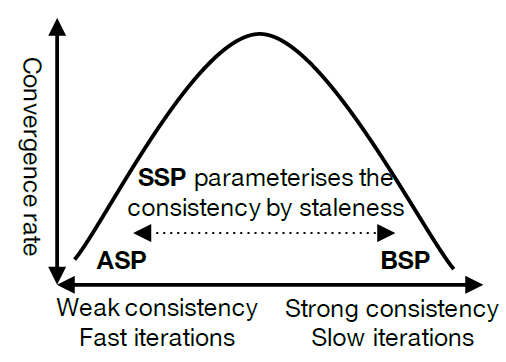
\includegraphics[scale=0.6]{Pic26.png}
		\caption{مقایسه سه مکانیزم کنترل مانع \cite{Zhao2021}}
		\label{p26}
	\end{center}
\end{figure}

همان‌طور که قبلا اشاره شده است، \lr{BSP} یک مدل محاسباتی موازی همه‌منظوره است که به‌طور موفقیت‌آمیز برای یادگیری توزیع‌شده به‌کار گرفته شده است. یکی از مشکلات رایج مدل \lr{BSP} کلاسیک این است که در هر تکرار همه گره‌ها ملزم به انتظار برای کند‌کننده\footnote{\lr{Straggler}}  می‌باشند. به طور قطع در یک کلاستر بزرگ برای یادگیری توزیع‌شده، گره‌ها با سخت‌افزار متفاوت و ظرفیت‌های پویا وجود خواهند داشت. در نتیجه تنگنای اصلی در چنین روش‌هایی ناشی از مساله کند‌کننده‌ها است. به طور معمول کند‌کننده در یک محیط ناهمگنی وجود دارد که سرعت پردازش و قدرت محاسبات گره‌ها در آن متفاوت است. در یک محیط همگن نیز ممکن است کند‌کننده وجود داشته باشد، که ناشی از عدم تعادل بار بین گره‌ها، کندی تصادفی یک گره یا تاخیر در لینک ارتباطی است. تاخیر لینک ارتباطی به دلیل یکی از دو منبع ارتباطات درونی و بین کامپیوتری خواهد بود. 

برای مقابله با مساله کند‌کننده‌ها در شبکه یادگیری توزیع‌شده، در مقاله \cite{Mitigating2020} یک پروتکل به نام \lr{RNA}\footnote{\lr{Randomized Non-blocking AllReduce}} مبتنی بر الگوریتم غیرمتمرکز \lr{AllReduce} جزئی برای مدیریت کلاسترهای ناهمگن پیشنهاد شده است. در این پروتکل، یک گره آغازگر به صورت تصادفی از بین گره‌های دیگر انتخاب می‌شود. زمانیکه کار گره آغازگر تمام می‌شود، صرف نظر از اینکه سایر گره‌ها محاسبات شان را تمام کرده باشند یا خیر، عمل کاهش در کل شبکه انجام می‌شود. 

پروتکل به‌روزرسانی در \lr{BSP} دقت همگرایی بالا دارد اما بازده یا سرعت یادگیری متناظر با آن در حضور کند‌کننده‌ها تحت تاثیر منفی قرار می‌گیرد. درحالیکه \lr{APS} سرعت یادگیری بالاتری دارد اما دقت و همگرایی آن تحت تاثیر منفی گرادیان‌های کهنه قرار می‌گیرد. در \cite{Syncswitch2021} یک روش همگام‌سازی ترکیبی به نام \lr{Sync-Switch} با بهره‌گیری از مزایای \lr{BSP} و \lr{ASP} ارائه شده است که با کاهش زمان یادگیری به طور همزمان دقت همگرایی را حفظ می‌کند. از یک سری سیاست‌های تطبیقی برای تعیین چگونگی و زمان جا‌به‌جایی بین دو پروتکل‌ همگام‌سازی استفاده کرده‌اند. بدین منظور ترکیب‌های مختلف پروتکل \lr{ASP} و \lr{BSP} با توجه به دقت همگرایی مورد ارزیابی قرار گرفته است. در بهترین حالت، فرایند یادگیری با پروتکل همگام‌سازی \lr{BSP} آغاز می‌شود و در صورت برقراری یکی از شرایط 1) رسیدن به یک دقت همگرایی مشخص یا 2) به‌وجود آمدن کند‌کننده‌های گذرا در کلاستر یادگیری، به پروتکل همگام‌سازی \lr{ASP} جابه‌جا می‌شود. در این مقاله نشان داده شده است که یادگیری با \lr{BSP} برای 50 درصد از بارکاری و سپس یادگیری با \lr{ASP} بر روی باقی‌مانده بارکاری در مقایسه با ترکیب‌های دیگر نتایج بهتری را ارائه می‌دهد. شکل \ref{p27} ترکیبات مختلف دو مکانیزم کنترل مانع \lr{ASP} و \lr{BSP} را نشان می‌دهد. 

\begin{figure}[h]
	\begin{center}
		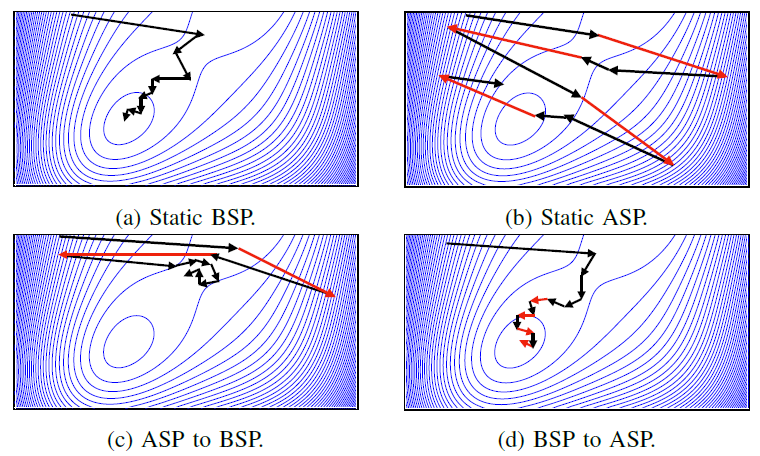
\includegraphics[scale=0.6]{P27.png}
		\caption{ترکیبات مختلف \lr{BSP} و \lr{ASP} بر روی یک تابع هزینه ساده \cite{Syncswitch2021}}
		\label{p27}
	\end{center}
\end{figure}

در الگوریتم گرادیان کاهشی تصادفی دسته‌ای \lr{(Minibatch SGD) } هر گره گرادیان را با استفاده از داده‌های محلی خودش محاسبه کرده و سپس گره‌ها گرادیان‌های محلی‌شان را میانگین می‌گیرند و از گرادیان حاصل برای به‌روزرسانی نهایی استفاده می‌شود. الگوریتم گرادیان کاهشی تصادفی محلی (\lr{Local SGD}) به عنوان بهبودی بر الگوریتم دسته‌ای پیشنهاد شده است. در این الگوریتم در هر دور هر گره \lr{K} گام از \lr{SGD} را بر روی هدف محلی و داده‌های خودش اجرا می‌کند. در نهایت نتایج به‌روزرسانی گره‌ها به عنوان نتیجه نهایی آن دور میانگین‌گیری می‌شود. در محیط‌های همکن و نزدیک به همگن نسخه محلی بر دسته‌ای غلبه می‌کند. در \cite{Minibatch2020} کارایی این دو نسخه در محیط‌های ناهمگن مورد بررسی قرار گرفته است. آنها نشان دادند که با تغییر تنظیمات از همگن به ناهمگن، کارایی نسخه محلی به طور قابل توجهی کاهش پیدا می‌کند. 

همان‌طور که ذکر شد، الگوریتم گرادیان کاهشی تصادفی محلی برای همه سناریوها قابل اجرا نیست. گره‌ها ممکن است از نظر قابلیت‌های محاسباتی ناهمگن باشند و زمان مورد نیاز برای یادگیری محلی گره‌ها یکسان نیست. به همین دلیل یادگیری کاملا همزمان گره‌ها ممکن است پرهزینه یا حتی غیرممکن باشد. اکثریت قریب به اتفاق کارهای ارائه شده یک مدل همزمان استفاده می‌کنند که در آن همه گره‌ها قبل از ارسال به‌روزرسانی‌هایشان به سرور مرکزی، با تعداد تکرار یکسانی آموزش می‌بینند. همچنین در بیشتر کارهای انجام‌شده مدل ارتباطی \lr{Hub-and-Spoke} فرض می‌شود، اما این مدل بسیاری از حالت‌های دنیای واقعی را نشان نمی‌دهد. به عنوان مثال، دستگاه‌های موجود در یک شبکه اقتضایی متحرک به دلیل محدودیت‌های شبکه یا محدوده ارتباطی، ممکن است همه نتوانند در یک گام با سرور مرکزی ارتباط برقرار کنند. در چنین حالتی، یک مدل شبکه ارتباطی چند سطحی مناسب است. 

در \cite{zhou2019} الگوریتمی به نام \lr{SGD} محلی سلسله مراتبی \lr{ (HL-SGD)} برای یادگیری مدل در یک شبکه سلسله مراتبی با توپولوژی \lr{Hub-and-Spoke} پیشنهاد شده است و همه گره‌های شبکه همگن فرض شده‌اند. تحلیل خطا همگرایی و زمان همگرایی الگوریتم \lr{HL-SGD } در \cite{Liu2020, Abad2020} برای یادگیری فدرالی\footnote{\lr{Federated Learning}} بحث شده است. الگوریتم \lr{SGD} محلی چندسطحی \lr{MLL-SGD} \cite{MLL2020} یک الگوریتم یادگیری توزیع‌شده برای شبکه‌های سلسله مراتبی با گره‌های ناهمگن است. در این الگوریتم، ساختار شبکه به صورت دو سطحی در نظر گرفته شده است. سطح پایین‌تر شامل مجموعه‌ای از شبکه‌های فرعی \lr{Hub-and-Spoke } است که هر کدام دارای یک سرور هاب و مجموعه‌ای از گره‌ها است. شبکه سطح بالا شامل یک شبکه هاب متصل که توسط آن هاب‌ها با هم ارتباط برقرار می‌کنند. هر شبکه فرعی چند دور \lr{SGD} محلی را اجرا می‌کند. بعد از یک دوره آموزش محلی گره‌ها، در مرکز شبکه فرعی میانگین‌گیری مدل انجام می‌شود. به طور دوره‌ای، هاب‌ها مدل‌های خود را با همسایگان در شبکه هاب میانگین‌گیری می‌کنند. 

مکانیزم‌های کنترل مانع در الگوریتم‌های یادگیری تکراری نقش بسیار حیاتی را ایفا می‌کنند. در اغلب محاسبات داده-موازی، پارامترهای مدل اشتراکی براساس به‌روزرسانی‌های جداگانه از هر قطعه داده به‌روز می‌شوند. به عبارت دیگر، به‌روزرسانی‌های تجمیع‌شده برای به‌روزرسانی مدل استفاده می‌شوند. به‌روزرسانی‌های همگام نشده باعث ایجاد خطا و نویز در مدل نهایی خواهند شد. 

در یک محیط بسیار نامطمئن، لینک‌ها ممکن است خراب شوند و پهنای باند ناهمگن است؛ همچنین گره‌ها ثابت نیستند، می‌توانند در هر زمان به سیستم بپیوندند و یا از آن خارج شوند. بنابراین، در چنین محیطی با تضمین اینکه اکثر سیستم‌ها دارای مرز همگام‌شده هستند، می‌توان این تأثیرات را به حداقل رساند. میزان همگام‌سازی یک مانع نشان‌دهنده‌ی مبادله بین دقت (در هر تکرار) و کارایی (سرعت همگرایی) یک الگوریتم یادگیری تکراری است. با توجه به مزایا و معایب هر مکانیزم همگام‌سازی، \lr{BSP} قطعی است و می‌تواند به همان طراحی الگوریتم یادگیری ماشین منجر شود. مکانیزم‌های قطعی نظارت و کنترل همگام‌سازی مانع در یک محیط بسیار پویا ممکن است مناسب نباشند. در مقاله \cite{wang2017} یک تکنیک کنترل مانع احتمالی به نام \lr{PSP}\footnote{\lr{Probabilistic Synchronous Parallel}} بر اساس یک نمونه‌گیری اولیه ارائه شده است که در مقایسه با سه تکنیک کنترل مانع رایج در یک سیستم بسیار پویا و خیلی بزرگ به طور موثر سرعت همگرایی و مقیاس‌پذیری الگوریتم گرادیان کاهشی تصادفی را بهبود می‌بخشد. همگام‌سازی مانعی در تکنیک \lr{PSP} به روش احتمالی کنترل می‌شود، یعنی با نمونه‌برداری از گره‌های شرکت‌کننده در یادگیری درصدی از گره‌های سیستم که مرحله فعلی را به پایان رسانده‌اند را تخمین می‌زند. ایده اصلی مکانیزم \lr{PSP} این است که ما نیاز داریم که فقط بخشی از گره‌ها نه همه آنها، در پروسه همگام‌سازی قرار بگیرند. روش‌های موجود کنترل همگام‌سازی مانع و سازگاری مدل را تجمیع می‌کنند، درحالیکه \lr{PSP} کنترل همگام‌سازی مانع را از سازگاری مدل جدا می‌کند. 

در یادگیری فدرال، گره‌های توزیع‌شده و ناهمگن برای یادگیری پارامترهای مدل با یکدیگر همکاری می‌کنند. با این‌حال، در حالی که مزایایی مانند حفظ حریم خصوصی با طراحی و کاهش تأخیر ایجاد می‌کند، شبکه ناهمگن چالش‌هایی را برای روش‌های همگام‌سازی یا روش‌های کنترل موانع، در مورد پیشرفت سیستم و همگرایی مدل و غیره ایجاد می‌کند. در \cite{Zhao2021} از مکانیزم \lr{PSP} برای یادگیری فدرال استفاده شده است و آنها پیشنهاد دادند که می‌توان مکانیزم‌های موجود، به ویژه \lr{BSP} و \lr{SSP}، را برای ایجاد مکانیزم‌های کنترل مانع کاملاً توزیع‌شده و مقیاس‌پذیرتر ترکیب کرد. این کار سبب می‌شود که با بزرگتر شدن سیستم به منظور جلوگیری از خفه شدن سرور و عدم ایجاد تنگنا، ارتباطات بین گره‌ها و سرور کاهش یابد. در شکل \ref{p28} مکانیزم احتمالی \lr{PSP} با \lr{BSP} ترکیب شده است و در نمونه‌برداری اولیه انجام شده از گره‌های موجود در سیستم، مکانیزم کنترل مانع \lr{BSP} اجرا شده است.


\begin{figure}[h]
	\begin{center}
		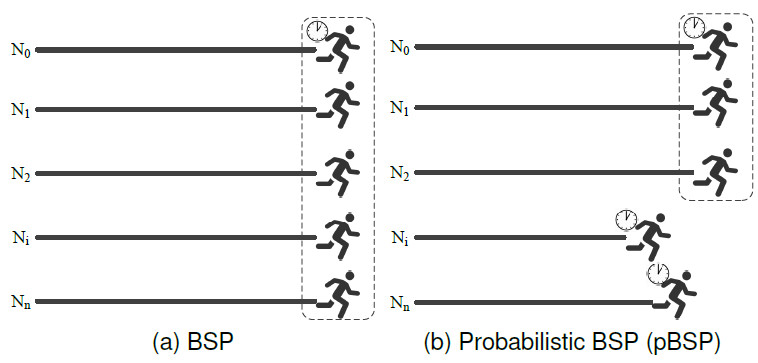
\includegraphics[scale=0.6]{P28.png}
		\caption{ترکیب \lr{PSP} با مکانیزم کنترل مانع \lr{BSP} \cite{wang2017}}
		\label{p28}
	\end{center}
\end{figure}

برای رفع نیاز به همگام‌سازی دقیق در مکانیزم \lr{BSP} و کاهش زمان انتظار گره‌های سریع در مقاله \cite{zhao2020elastic} یک روش همگام‌سازی الاستیک یا قابل ارتجاع به نام \lr{ElasticBSP} پیشنهاد شده است. این روش همکام‌سازی مبتنی بر یک الگوریتم به نام \lr{ZipLine} است که زمان اجرای همگام‌سازی را تخمین می‌زند. در مرحله اول برای هر گره نقاط پایانی در تکرارهای آینده در زمان اجرا تخمین زده می‌شوند و در مرحله دوم یک الگوریتم تک-گذر بر روی نقاط پایانی تخمین زده شده‌ی همه گره‌ها اجرا می‌شود تا یک نقطه زمانی بهینه در تکرار بعدی برای همگام‌سازی به صورت سریع محاسبه گردد. 

هدف این روش تسهیل شرایط همگام‌سازی دقیق مکانیزم \lr{BSP} برای کاهش زمان انتظار گره‌ها و در نتیجه افزایش توان تکرارها، و در عین حال محدود کردن گرادیان‌های قدیمی و مقادیر قدیمی آنها در روند همگرایی الگوریتم گرادیان کاهشی تصادفی تکراری است. همچنین در مقایسه با مکانیزم \lr{SSP}، مدل پیشنهادی ظرفیت محاسباتی گره‌ها را در نظر می‌گیرد. بنابراین انعطاف‌پذیری و سازگاری بیشتری را در طول مرحله یادگیری بدون کاهش دقت مدل آموزشی، ارائه می‌دهد. 

در روش \lr{ElasticBSP}، زمان اعمال مانع همگام‌سازی متفاوت است و هر ابرگام تعداد متفاوتی از تکرارها را برای هر گره مجاز می‌کند. این مقادیر در زمان اجرا توسط الگوریتم \lr{ZipLine} تعیین می‌شوند که حداقل زمان انتظار کلی همه گره‌ها را به دست می‌آورد. شکل \ref{p2930} به خوبی تفاوت زمان اجرای ابرگام‌ها در \lr{BSP} و \lr{ElasticBSP}  در یک شبکه با 4 گره را نشان می‌دهد. در هر ابرگام قسمت رنگی هر گره زمان محاسبات و قسمت سفید رنگ زمان ارتباطات را بیان می‌کنند.
%\iffalse
\begin{figure}
	\centering
	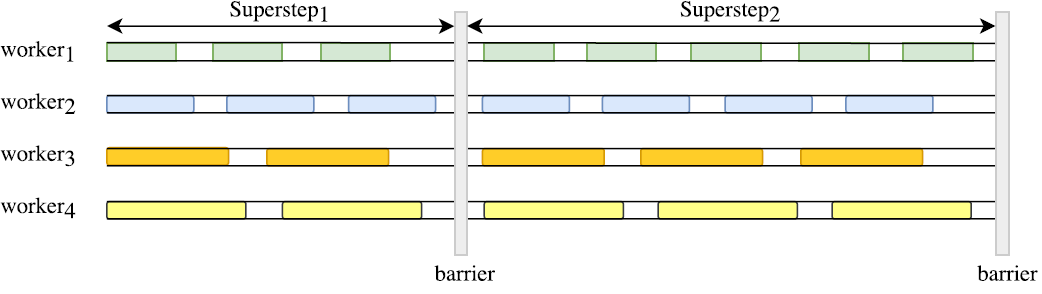
\includegraphics[width=\textwidth]{Pic29.png}
	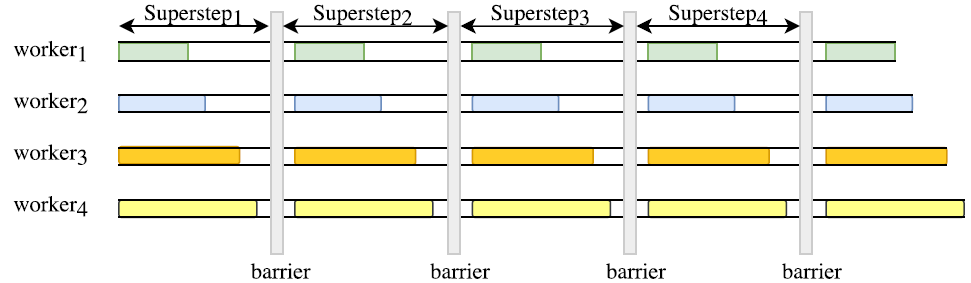
\includegraphics[width=\textwidth]{Pic30.png}
	\caption{تفاوت زمان اجرای ابرگام‌ها در \lr{BSP} و \lr{ElasticBSP} \cite{Zip2021}}
	\label{p2930}
\end{figure}
%\fi


\subsection{کاهش هزینه سربار ارتباطی در الگوریتم‌های توزیع‌شده}

سربار ارتباطی به عنوان گلوگاه اصلی در الگوریتم‌های \lr{SGD} داده- موازی شناسایی شده است. موازی‌سازی داده‌ها به صورت خطی قدرت پردازش را توسط محاسبات گرادیان همزمان با چندین پردازنده افزایش می‌دهد. الگوریتم‌های \lr{SGD} مبتنی بر \lr{BSP} به عملیات ارتباط جمعی بسیاری از جمله، پخش پارامترها یا تجمیع گرادیان‌های جزئی نیاز دارند. این عملیات نیاز به همگام‌سازی دارند. این عملیات برای پیام‌های بزرگ به شدت بر زمان اجرای کلی تاثیر می‌گذارند و مقیاس‌پذیری موازی را محدود می‌کنند. پیام‌ها در آموزش شبکه‌های عصبی در مقیاس بزرگ متراکم، طولانی و با طول ثابت هستند، در حالی که عملکرد الگوریتم‌های جمعی به شدت به این ویژگی‌ها حساس است. از آنجایی‌که در عمل، سرعت ارتباط چندین مرتبه کندتر از سرعت پردازش و محاسبه است. در طراحی و به‌کارگیری عملیات جمعی باید پهنای باند شبکه در اولویت قرار گیرد. در ادامه این بخش تعدادی از رویکردها برای کاهش سربار ارتباطی پیشنهاد شده است.  

اولین دسته از رویکردهای پیشنهادی برای افزایش توان عملیاتی تکرار مدل‌های همزمان \lr{SGD} را تسهیل می‌کنند \cite{Zin2010,NIPS2012} در این مورد، \lr{SGD} تسهیل‌شده محاسبات روی یک پردازنده را قادر می‌سازد تا حدی با ارتباطات روی سایر پردازنده‌ها همپوشانی داشته باشد. رویکرد \lr{ASP} یک \lr{SGD} غیرهمزمان بدون قفل را پیشنهاد می‌کند \cite{Hog12011}  که با اجازه‌دادن به به‌روزرسانی مستقل پارامترهای همزمان، به طور کامل از نیاز به همگام‌سازی رها شود. اما همگام‌سازی تسهیل‌شده فقط در مورد مسائل یادگیری خلوت به خوبی جواب می‌دهد. رویکرد \lr{SSP} مفهوم کهنگی را برای اطمینان از صحت و درستی معرفی می‌کند \cite{Ho2013} که برای این منظور میزان فاصله سریعترین و کندترین گره‌ را بر اساس تعداد تکرار از یکدیگر محدود می‌شود. رویکردهای تسهیل‌شده ادعا می‌کنند که با افزایش توان عملیاتی تکرارها، نرخ همگرایی کاهش یافته را جبران می‌کنند. 

دسته دوم رویکردها سعی در کاهش حجم کلی ارتباطات دارند. در مقاله \cite{ّFrank2014} برای کاهش طول پیام، گرادیان از 32 بیت به 1 بیت کوانتیزه یا کمی می‌شود، اما اطلاعات گرادیان از دست‌رفته نرخ همگرایی را به شدت کاهش می‌دهد. روش دیگر، تسریع همگرایی با یک دسته بزرگ است. در مقاله \cite{dekel2012} اثبات شده است که نرخ همگرایی \lr{Mini-batch SGD } از مرتبه $O(1/\sqrt{Tb}+\frac{1}{T})$ است که $b$ اندازه دسته را نشان می‌دهد. رویکردها با دسته‌های داده بزرگ به تکرارهای کمتری برای یافتن راه حل نیاز دارد و در نتیجه همگام‌سازی‌های کلی کمتری نیاز دارد. در \cite{wang2017} نشان داده شده است که افزایش نامطلوب اندازه دسته‌ها تحت منابع محاسباتی محدود، نامطلوب است. این روش‌ها همچنان به همگام‌سازی نیاز دارند. 

دسته سوم رویکردها با بهینه‌سازی سیستم سعی در به حداقل رساندن هزینه ارتباطات دارند. در مقاله \cite{ag2011} تجمیع گرادیان‌های جزئی هدایت‌شده با یک \lr{MST}\footnote{\lr{Minimum Spanning Tree}} پیشنهاد شده است که به $log(P)$ گام برای همگام‌سازی کامل مدل نیاز دارند. چارچوب‌های یادگیری عمیق مانند \lr{Caffe} نیز این رویکرد را بکار می‌گیرند. متأسفانه، \lr{MST} فقط برای سناریوهایی با پیام‌های کوتاه و پرتکرار مناسب است. کارایی عملیات جمعی در این روش به طور قابل توجهی با طول پیام‌ها و توپولوژی‌های شبکه تغییر می‌کند. در حالی‌که پیام‌ها در آموزش شبکه عمیق متراکم، طولانی و با طول ثابت هستند. بنابراین، رسیدگی به چنین ویژگی‌هایی در عملیات جمعی ضروری است. در مقاله \cite{Pip2003} یک مدل جمعی خط ‌لوله در محیط حافظه اشتراکی برای داده‌های \lr{CPU} ارائه شده‌ است. اما ارتباطات فرآیندهای مختلف \lr{MPI} یک گذرگاه حافظه \lr{CPU} را در یک سوکت \lr{CPU} به اشتراک می‌گذارند. این باعث رقابت پهنای باند بین فرآیندهای مختلف می‌شود و در نتیجه عملکرد ضعیفی برای ارتباطات جمعی در محیط حافظه مشترک برای داده‌های \lr{CPU} ایجاد می‌کند.

جدیدترین پردازنده‌های گرافیکی دارای دو موتور \lr{DMA} مستقل برای ارتباطات ورودی/خروجی مستقل هستند. بر این اساس، در مقاله \cite{Zhao2017} تکنیکی به نام خط‌لوله خطی (\lr{LP}) مبتنی بر عملیات جمعی برای آموزش چند پردازنده گرافیکی ارائه داده‌‌اند. در این طرح برای به حداکثر رساندن تبادل داده‌های دو‌طرفه همزمان، پیام‌ها به بلوک‌های ریزدانه به عنوان عنصر اصلی ارتباط تقسیم می‌شوند. یک \lr{GPU} یک بلوک (از طریق  1\lr{DMA}) ارسال می‌کند در حالی‌که (از طریق  2\lr{DMA} ) یک بلوک جدید از یک همسایه دریافت می کند. کپی‌ها به صورت غیرهمزمان بر روی دو جریان \lr{GPU} قرار می‌گیرند و عملیات عددی بیشتر با کپی‌های داده همپوشانی دارند. از این طریق، خط‌لوله بسیار کارآمدی برای رد و بدل پیام‌های آموزش شبکه عصبی دردسترس خواهد بود. تکنیک خط‌‌‌لوله خطی باعث افزایش تسریع به اندازه $O(Log P)$ نسبت به عملیات جمعی \lr{MST} و باعث افزایش به اندازه دو برابر نسبت به روش‌های مبتنی بر \lr{BE} می‌شود. ویژگی مهم این تکنیک این است که هزینه طراحی آن نسبت به تعداد \lr{GPU}ها ثابت است، یعنی هزینه عملیات جمعی روی دوتا پردازنده گرافیکی شبیه به هزینه عملیات جمعی بر روی بیست‌تا پردازنده گرافیکی است. شکل \ref{p25} نحوه عملکرد سه عملیات جمعی در تکنیک خط‌لوله خطی بر روی سه پردازنده گرافیکی را نشان می‌دهد. 
\begin{figure}[h]
	\begin{center}
		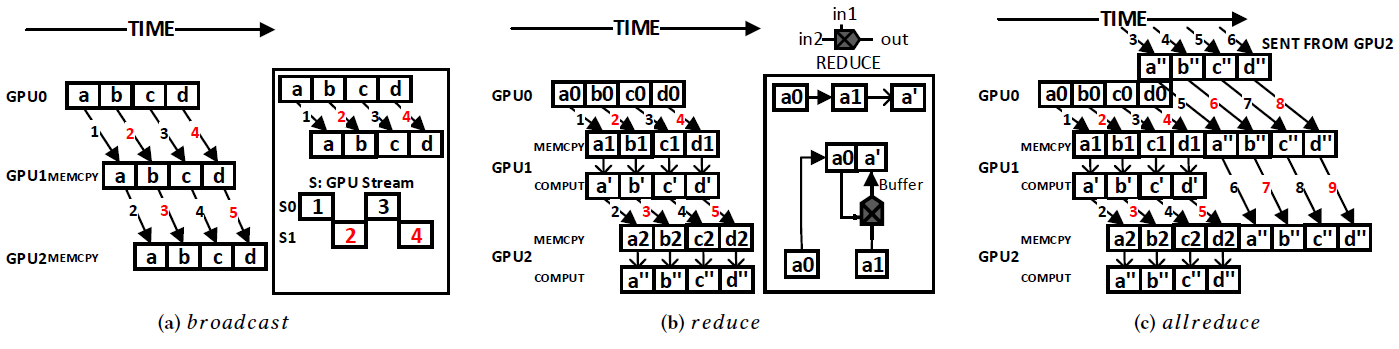
\includegraphics[scale=0.4]{Pic25.png}
		\caption{جریان‌داده عملیات پخش، کاهش و همه‌کاهش بر روی سه پردازنده گرافیکی \cite{Zhao2017}}
		\label{p25}
	\end{center}
\end{figure}


الگوریتم مرتبه دوم \lr{AsySQN} \cite{tong2020} یک الگوریتم موازی غیرهمزمان براساس روش شبه نیوتن تصادفی است که مبتنی بر یک پلتفرم حافظه اشتراکی برای حل مسائل بدشرط ارائه شده است. در الگوریتم \lr{AsySQN} براساس تکنیک‌های حافظه مدرن، از قفل‌هایی استفاده می‌شود که تضمین می‌کند در هر لحظه فقط یک پردازنده می‌تواند در حافظه اشتراکی بنویسد. بدین منظور یک تایمر سراسری \lr{t} بکار گرفته می‌شود و زمان‌های به‌روزرسانی حافظه اشتراکی را ذخیره می‌کند. در الگوریتم غیرهمزمان، هنگامی‌که یک پردازنده در حال به‌روزرسانی پارامتر مشترک \lr{x} به $x_t$ است، پردازنده دیگر هنوز وضعیت قدیمی پارامتر $x_{D(t)}$ برای به روزرسانی و محاسباتش استفاده می‌کند. در اینجا $D(t)\in [t]$ حالت خاصی از پارامتر مشترک \lr{x} برای یک رشته یا پردازنده در زمانی است که $x$ در زمان $t$  به‌روز شده است. به منظور حفظ کارایی روش، حداکثر تاخیر بین فرآیندها به صورت $t-D(t)\le \tau$ محدود شده است. رابطه به‌روزرسانی استفاده شده در این روش در رابطه \ref{e22} بیان شده است.
\begin{equation}\label{e22}
	x_{t+1}=x_t-\eta H(x_{\hat{D}(t)})\nu(x_{\hat{D}(t)})
\end{equation}


\section{خلاصه}
در این فصل به مرور مطالعات انجام شده در زمینه الگوریتم‌های یادگیری توزیع‌شده پرداخته شده. به طور کلی این مطالعات، به سه دسته کلی تقسیم گردید: در دسته اول و دوم به بررسی الگوریتم‌های یادگیری توزیع‌شده انتشاری در شبکه‌های تطبیقی و الگوریتم‌های یادگیری فدرالی متمرکز و غیرمتمرکز پرداخته شد و دسته سوم شامل روش‌های موازی‌سازی الگوریتم‌های گرادیان کاهشی توزیع‌شده و الگوریتم‌های توزیع‌شده مبتنی بر مدل‌های محاسباتی موازی بود. 